%% uctest.tex 11/3/94
%% Copyright (C) 1988-2004 Daniel Gildea, BBF, Ethan Munson.
%
% This work may be distributed and/or modified under the
% conditions of the LaTeX Project Public License, either version 1.3
% of this license or (at your option) any later version.
% The latest version of this license is in
%   http://www.latex-project.org/lppl.txt
% and version 1.3 or later is part of all distributions of LaTeX
% version 2003/12/01 or later.
%
% This work has the LPPL maintenance status "maintained".
% 
% The Current Maintainer of this work is Daniel Gildea.

\documentclass[11pt]{ucthesis}
\def\dsp{\def\baselinestretch{2.0}\large\normalsize}
\dsp

% 2010june01 sol katzman:
% package geometry should override the various margin settings from .clo and .cls
% and also eliminates issues where the default papersize is A4
\usepackage[letterpaper, left=1.5in, right=1.25in, top=1.25in, bottom=1.25in, includefoot]{geometry}

\usepackage{url}
\usepackage{listings}
\usepackage{graphicx}
\usepackage{xspace}
\usepackage{amsmath}

\begin{document}

% Have a command for vocab words
\newcommand{\vocab}[1]{\textbf{#1}\xspace}

% Declarations for Front Matter

\title{Infrastructure for Scalable Analysis of Genomic Variation}
\author{Adam M. Novak}
\degreeyear{2017}
\degreemonth{June}
\degree{DOCTOR OF PHILOSOPHY}
\chair{Professor Josh Stuart}
\committeememberone{Distinguished Professor David Haussler}
\committeemembertwo{Assistant Professor Ed Green}
\committeememberthree{Associate Professor Beth Shapiro}
\numberofmembers{4} %% (including chair) possible: 3, 4, 5, 6
\deanlineone{Dean \textbf{Tyrus Miller}}
\deanlinetwo{Vice Provost and Dean of Graduate Studies}
\deanlinethree{}
\field{Bioinformatics}
\campus{Santa Cruz}

\begin{frontmatter}

\maketitle
\copyrightpage

\tableofcontents
\listoffigures
\listoftables

\begin{abstract}
    Bioinformatics thinks too small. If we are to effectively engage with human biology, we need to be able to think on scales of millions or billions of individuals. Unfortunately, the software tools that we use to analyze the human genome, and indeed the very concept of a unified ``the human genome'', start to break down at such scales. In order to remedy this, I propose a three-part research agenda: creating a new conceptual framework for using graphs as pluralistic genomic references, implementing scalable software tools for shared infrastructure to build and operate on such graphs, and applying these tools to solve previously difficult problems in genomics.
\end{abstract}

\begin{acknowledgements}
In addition to my advisor Prof. David Haussler, and the other members of my committee, I would like to thank Dr. Benedict Paten for helping to direct my research efforts, Yohei Rosen for collaborating with me on mapping algorithms, Frank Nothaft for his help with Spark and Avro, and everyone on the NOTCH2NL project. I would also like to thank Anna Henderson for her contributions as an editor.
\end{acknowledgements}

\end{frontmatter}

\chapter{Introduction}

Biology happens at scale. Scale, in population and in time, gives evolution the raw material it needs to shape biological systems worth studying. Scale enables bacteria to become resistant to antibiotics. Scale allows cancer to arise with alarming regularity in healthy people. Scale powers the adaptive immune system, and simultaneously enables pathogens to evade it. To really understand biological systems, we need to be able to match their scale.

In recent years, the scale of biological data collection has dramatically increased (in part due to a precipitous drop in the cost of DNA sequencing) \cite{wetterstrand2014dna}. Unfortunately, data collection has scaled up disproportionately along the ``number of features'' axis, and only moderately along the ``number of samples'' axis. The Cancer Genome Atlas (TCGA), for example, has collected many types of data, including genomic DNA sequences, DNA methylation data, and mRNA expression levels, amounting to millions of features per sample \cite{tcga2014sample}. However, TCGA has looked at a number of individual people and cancers only on the order of thousands \cite{tcga2014sample}. Similarly, while the 1000 Genomes Project found millions of unique genomic variants, it sampled only on the order of a thousand individuals \cite{10002010map}. While such sample sizes may sound large to those who remember the years of effort and multi-billion-dollar expenditure required by the original Human Genome Project, they are woefully small compared to the numbers of features per sample. From a machine learning perspective, this limits the amount of useful knowledge that can be extracted from all of that data \cite{hua2005optimal}. If a theory is to be expected to generalize to new data (that is, if it is to actually reflect the biological processes at work), it generally ought to be based on more data points than features \cite{hua2005optimal}.

For now, it is still possible to use such small sample sizes to do meaningful biology \cite{weinstein2013cancer}. However, at some point in the future, we will exhaust what we can learn by combining our prior knowledge of genetics and biochemistry with a few thousand high-throughput sequencing samples, and we will need to scale up enrollment.

Unfortunately, to scale sample sizes by even a few orders of magnitude, basic bioinformatics practices will need to change. As it is, working on huge datasets like the sequencing reads from TCGA is an enormous technical challenge, with thousands of gigabytes of data to transfer, store, and protect from unauthorized access. At some point, as we increase the number of samples, we will have to abandon the idea that every lab that wants to analyze these enormous community data sets ought to have its own local copy.

Additionally, when we start to scale up to large numbers of samples, our data sets are more likely to contain individuals who are in some way out of the ordinary, and consequently our engineering standards need to be tightened. For example, if a bioinformatics analysis pipeline assumes that a certain run of genes occur in a certain order and orientation, an increased number of samples pushed through this pipeline translates into an increased chance of encountering an individual who has a rearrangement contradicting that assumption. This will at best result in a run-time error and an unhappy bioinformaticist, and at worst a subtly incorrect result in a published paper. All the corner cases---the pathological combinations of variants that we assume won't co-occur, or the genomic regions that we would rather not talk about---need to be found and addressed if we are to scale up bioinformatics analyses to truly useful sizes.

This means that in order to scale up bioinformatics, we will need to solve a software quality problem. Software needs to be more robust to handle a million samples than to handle a thousand samples. One way to achieve this level of reliability would be to make every bioinformaticist a good software engineer. A more practical approach would be to provide bioinformaticists with good software libraries, which contain abstractions that can safely be applied to large numbers of samples, and which consistently expose the now-relatively-frequent edge cases which bioinformaticists will need to deal with at these scales. This latter approach is the one that I will take.

One of the abstractions which cannot be safely applied at these scales is the idea of a universal human reference genome and its associated linear coordinate space. Unfortunately, this idea is central to current bioinformatics practice. When you have only one sequenced genome, it's perfectly reasonable to, say, extract a 2 kilobase window of sequence centered on an arbitrary position. However, we now have thousands of sequenced genomes---enough to get a sense of what common variants exist in the human population, although not enough to understand the significance of many of them \cite{10002010map}---and it is growing increasingly clear that operations like windowing in the reference don't always make sense. For example, in the latest release of the human reference genome, GRCh38, there are 261 ``alt loci''---pieces of sequence which are not on the main reference chromosomes, but which model common alternative arrangements of genes and other genomic elements \cite{karolchik2014new}. In genomic regions where these alt loci apply, the traditional linear coordinate system, which refers to locations in peoples' genomes by the chromosome and base index in the reference genome, begins to break down. To properly reason about such genomic regions, we need to abandon either the idea that bases in peoples' genomes correspond to bases in a reference, or the idea that references are linear.

% TODO: Note about alt loci messing up mapping. Can I demo this or something?

The linear organization of the reference genome also frustrates attempts to study regions of the genome which are difficult to assemble, or which, due to sequence similarity, are very difficult to distinguish from similar regions at other locations in the genome. To facilitate analysis of the centromeres, for example, GRCh38 includes plausible synthetic linear centromere sequences \cite{karolchik2014new}. We have more precise, graph-based models of what we actually know about the centromeres, but these models cannot be indexed by linear sequence coordinates or processed by tools that expect a linear reference sequence \cite{miga2014centromere}.

I propose a nonlinear, graph-based ``reference structure'' for human genomes. A graph-based reference structure can capture in a first-class way the sequence information which is currently relegated to alt loci, as well as additional variant information from other sources. Combined with a rigorous definition of mapping sequencing reads to paths in the graph, a reference structure could potentially combat allele-specific mapping bias, an effect in which alleles that match the single linear reference are easier to detect than those which do not \cite{degner2009effect}. Furthermore, a hierarchy of reference structures could eventually allow for ``collapsing'' ambiguous regions together, with variable stringency, permitting the inclusion of a more accurate representation of our knowledge of centromeres and other repetitive or ambiguous regions of the genome.

For my thesis project, I will formalize the mathematics of constructing and mapping to a graph-based reference, build scalable software tools and API infrastructure for creating and working with reference structures and hierarchies, and use a constructed reference of this form to reach new, biologically relevant conclusions.

% Biology only works at scale

    % Scale in population and in time is what allows evolution to work
    
    % Scale produces drug resistance in bacteria
    
    % Scale produces cancer in healthy people
    
    % We won't be able to understand biology until we can match its scale

% High throughput is along the wrong dimension (so far)
    
    % We have a lot of features of a few samples.
    
    % To some extent we can get by with clever algorithms and educated guesses as prior knowledge.

% We need to be able to handle millions or even billions of samples if we want to be able to do biology just by looking.

    % Cancer, for example, won't make sense until we do this
    
% We need to be able to do this with something not millions of times better than current computing hardware

     % Because the transistors are now nearly as small as the stuff we're sequencing

% We can't scale that big by pushing BAM files around.

    % A billion 100-gig BAM files is 93 exabytes. That is too big to download.

% 1 in a million things start to happen, and we need infrastructure to handle them
    
    % We need to handle overlapping variants
    
    % We can't just throw out the alternate haplotypes
    
    % Assuming that everyone is contiguous in reference genome coordinates is going to get us into trouble
    
    % We can't keep messing around with the reference coordinates because we can't keep re-mapping every single read ever read.
    
    % We'll want to look at important variation in repetitive areas, and we may not yet have long reads

% So I'm going to build some stuff we will need in order to make this work
    
    % A non-linear coordinate system with stable base identifiers
    
    % A reference graph
    
        % Can capture more than just a single reference sequence
        
        % Reduce mapping bias
        
        % Probably less racist
        
    % A deterministic way to identify observed bases within that graph
        
    % A hierarchy of different versions of this graph with differing levels of specificity
        
        % Interlinked so you can project up and down for a rigorous notion of multimapping
        
% Then I'm going to try it out and discover something useful.
        
\chapter{Background}

\section{How Bioinformatics Works}

In my experience, there is a single workflow underlying most of what bioinformaticists do all day. It has three steps:

\begin{enumerate}
\item \textbf{Download} the data that you want to work with.
\item \textbf{Store} that data on your computer.
\item \textbf{Analyze} the data to reach scientific conclusions.
\end{enumerate}

While most researchers are concentrating on the last step of this process, as the datasets have grown the first two steps have become nontrivial problems. Take for example the case of the TCGA dataset, which has hundreds of Binary Alignment/Map (BAM) files of DNA sequence from tumor samples \cite{li2009sequence,tcga2014sample}. Each of these BAM files can be nearly a hundred gigabytes in size. In order for a lab to work with TCGA data, the lab needs to download a copy of it and store it in a secure environment which meets TCGA's access control standards.

Downloading tens of terabytes of data is not easy, and the problem is only going to get worse: the datasets to be downloaded are growing faster than the networks over which they are supposed to travel \cite{stein2010case}. Securely storing the downloaded datasets is even harder. This presents the greatest obstacle to smaller smaller labs without much computing infrastructure, but even large labs, like the Haussler Lab here at UCSC, have problems. One researcher in my lab managed to develop a data analysis anti-pattern wherein he would download one TCGA BAM file, analyze it, and then delete it, because he did not have sufficient secure storage space for the entire dataset he wanted to analyze. This is an enormous waste of time and bandwidth, and is not the sort of practice that we want to use as the foundation of sequence analysis.

The situation is only somewhat better for variation datasets than for sequence datasets. The 1000 Genomes Project variant data releases total about 500 gigabytes \cite{10002013release}. While this is certainly easier to download and store than tens of terabytes of read data would be, it's still much more than any scientist would want to carry around on their Macbook. It requires infrastructure to store, and that infrastructure gets duplicated at every institution that would like to analyze the data.

While these datasets might be manageable at their current sizes, on the order of a thousand samples, the same techniques are not going to be practical for long. In order to crack the really tough problems in bioinformatics, we need datasets with numbers of samples approaching or exceeding the number of features, which means millions or even billions of genomes. Such a dataset would be on the order of that stored by large corporations like Facebook, so it is not completely unreasonable to contemplate creating it \cite{anthony2012how}. It is unreasonable, however, to expect any single professor to pull in enough grant money to fund the storage of a billion whole genome BAM files. In order to scale up to the point where it is really useful, bioinformatics needs to transition to a shared-infrastructure model \cite{stein2010case}.

% How bioinformatics in general works

    % Download data
    
    % Analyze data
    
    % Already a huge pain with TCGA
    
        % Anyone who wants to work with the data needs a place to locally mirror it
        
        % And that place has to meet TCGA's exacting standards for data security and access control.
        
        % It would be much easier if TCGA could just do all the access control itself.
        
    % This is not going to be able to scale much bigger. Already it's very difficult for smaller labs to use these huge community data sets.

\section{Interactive Distributed Computing with Apache Spark}

In order to move bioinformatics to a shared-infrastructure model, we must build distributed bioinformatics tools. At least some of those tools should present interactive APIs accessible over the Internet; not every person who wants to make a query against shared infrastructure wants to write their own batch job to do it.

One useful tool for building distributed, interactive applications is Apache Spark. Spark is designed as an improvement on earlier batch-oriented map/reduce implementations which, while scalable to very large data sets, are fundamentally non-interactive \cite{zaharia2012fast,zaharia2012resilient}. In Spark, intermediate results and frequently-accessed data sets can be kept in memory across the nodes of the cluster instead of being spilled to disk \cite{zaharia2012fast,zaharia2012resilient}. This makes repeated queries, iterative computations, and cumulative pipelines much faster \cite{zaharia2012fast,zaharia2012resilient}. One of the major use cases of Spark is to provide an interactive terminal session for running queries on ``big data'' datasets \cite{zaharia2012fast,apache2014interactive}.

In Spark, distributed data is stored in the form of Resilient Distributed Datasets (RDDs), which permit distributed in-memory data structures to survive node failures \cite{zaharia2012resilient}. Since large pieces of computing infrastructure often suffer from individual node failures, which can force a na\"{\i}vely designed in-memory analysis pipeline to completely restart, this sort of fault tolerance is important \cite{thanakornworakij2013reliability}.

Spark is the centerpiece of a complete next-generation cluster infrastructure. For persistent storage of data on disk, Spark integrates with Apache Hadoop's Hadoop Filesystem (HDFS), which effectively distributes and replicates large data files across cluster nodes' disks \cite{zaharia2012fast,borthakur2008hdfs}. Spark works to schedule operations on on-disk data on the nodes where the data is actually stored, to prevent it having to be sent over the network \cite{borthakur2008hdfs}. HDFS allows disk I/O to be distributed, partially compensating for the relative slowness of access to spinning disks \cite{borthakur2008hdfs}. For cluster job control, Spark integrates with Apache's next-generation cluster resource manager Mesos, or Hadoop's next-generation built-in scheduler YARN \cite{apache2014cluster}.

Finally, while Spark is optimized for in-memory computing, it works perfectly well as a platform for batch jobs. Keeping commonly-accessed data in memory helps any job \cite{zaharia2012fast}. However, in-memory caching is particularly useful for jobs which need to iterate repeatedly on some intermediate state, such as machine learning pipelines \cite{zaharia2012fast}. This makes Spark, or a subset of or wrapper over Spark, a reasonable interface for people who \textit{do} want to make batch queries against shared infrastructure.

% We are moving to shared infrastructure for a reason, not just so we can throw our existing tools on someone else's machines

% The reason is that our data sets are getting too big to conveniently drag around with us

% We need to use something fancier than your everyday C/Python/Perl/Bash amalgamation that is your typical bioinformatics pipeline.

% We need tools that let us operate on large data sets in parallel, across many machines
    
    % Parallel storage
    
    % Parallel I/O
    
    % Parallel processing
    
% Apache Spark does this
    
    % Uses HDFS for parallel storage and I/O
    
        % Still need to replicate important data sets to different geographical/political/administrative regions to avoid things like someone blowing them up, but basically solves data loss due to disk failures.
        
    % Lets you specify iterative computations that happen in memory, distributed across your cluster.
    
    % With Mesos, multiple users can work on the same infrastructure against the same dataset.
    
    % Lets scientists interactively poke at data

\section{API Description with Avro}

Whereas bioinformatics practice has in the past centered around file formats as the interfaces between the different components of analysis systems, a move to shared infrastructure offers an opportunity, and in some ways creates a requirement, to rebuild the field on top of application programming interfaces (APIs) instead. If the idea is to use shared infrastructure and send the code to the data, then the code is going to have to know how to run on the shared infrastructure when it gets there, by being written against a standardized API. While any competent bioinformaticist can write a good-enough single-threaded FASTA (DNA sequence) parser, it is significantly harder to write a good enough distributed, parallel, fault-tolerant FASTA parser. In a system like HDFS, where parsing a file can be a complex distributed operation, user applications would be best off delegating that sort of work.

In addition to these sorts of internal APIs, a move to shared infrastructure will, as mentioned above, require creating external, higher-level query APIs, for the sorts of database searches and queries which do not necessarily merit spinning up an entire distributed processing pipeline.

One method to specify these APIs, and the complex data types which they need to exchange, is with the interface description language (IDL) of Apache Avro \cite{apache2014avro}. This language allows the specification of protocols through which applications can exchange messages and data with pieces of shared infrastructure \cite{apache2014avro}. Remote procedure call (RPC) code for accessing these APIs either within a cloud computing environment or over the Internet can be automatically generated in several popular languages \cite{apache2014avro}. If the resource happens to be local, it can be (at least in some target languages) accessed through the same generated interface. Avro descriptions of record structures can also be used to define on-disk file formats for data stored in HDFS, with parallel serialization and deserialization code also being generated automatically \cite{massie2013powerful}. 

An example Avro IDL is given below:

\begin{lstlisting}[basicstyle=\ttfamily, frame=single]
protocol Aligner {
    record Alignment {
        string gappedQuery;
        string gappedReference;
    }
    Alignment align(string query);
}
\end{lstlisting}

This IDL defines a protocol called \texttt{Aligner}, which has one remote call, \texttt{align}. The \texttt{align} function takes a single string, which is the sequence to align, and returns an \texttt{Alignment} record, which is defined as a pair of strings representing the alignment of the query to some reference.

% We want to standardize on APIs over file formats

    % Because things like reading a file are hard at scale
    
    % Because if you want to send the code to the data, the code needs to be able to interface with the system surrounding it at the other end
        
        % Not all queries are big enough to merit sending up entire VMs
        
        % Even a VM you sent up would need to pull data out of this fancy distributed data store, which is more complicated than opening a file
        
    % Replace "formats" with "schemas"
    
    % Enumerate RPC operations that code you send up is going to have
    
    % Or that the shared datastores will present to outside users for queries.
    
% One method for specifying these APIs, and the data types that they exchange, is with the Interface Description Language (IDL) Apache Avro.
    
    % It integrates well with Spark and Hadoop
    
    % You can specify an API and get code generation for an RPC implementation.

\section{How Genomics Works}

One piece of shared infrastructure that bioinformatics already uses is the human reference genome, which was built at great expense at the turn of the millennium and is maintained by the Genome Reference Consortium (GRC) \cite{church2011modernizing}. This reference genome assembly was originally created by stitching together actual observed pieces of DNA sequence into a single-copy haploid \vocab{golden path} representing a complete genome \cite{church2011modernizing}. Under this model, a hypothetical perfect assembly would have a single \vocab{contig}, or contiguous linear string of DNA bases, per chromosome. This naturally suggests a coordinate system: bases can be referred to by the contig they are on and their offset from the beginning of that contig.

This coordinate system is a critical piece of genomics infrastructure. It allows the reference genome to be annotated with genes and other elements. It provides the backbone to which descriptions of genomic variation are anchored. It defines the space in which genome sequencing happens, as short reads from sequencing machines are \vocab{mapped} to positions in this space. The entire field depends on this coordinate system.

Unfortunately, whenever the official human reference genome is updated, and bases are inserted or removed, the old coordinates are no longer valid on the new reference, and a period of mass confusion ensues as everyone who studies human genomics translates everything they are working on over to the new coordinate system, and then wonders whether their colleagues have done the same. Resources that aren't converted to the new system are at best lost to the field, and at worst applied inappropriately to the wrong genomic locations.

The golden path model is inextricably bound to the concept of ``the human genome''---the idea that one prototypical set of 24 chromosomes is a suitable foundation for the field of genomics. This idea has been central to human genomics, but it is not without its flaws. Putting aside the unfortunate normative implications of declaring the allele from whomever you sequenced first as ``reference'' and any alternatives from other populations as ``variant'', using a single reference genome when mapping sequencing reads leads to the well-known phenomenon of \vocab{reference bias}. Reads matching the reference genome at a variant site tend to map better and more often than those supporting differences from the reference. This reference bias affects many popular short-read aligners \cite{lunter2011stampy}. Additionally, in some genomic regions there are dramatically structurally distinct haplotypes present in the population \cite{church2011modernizing}. One example of this phenomenon is the extremely variable Major Histocompatibility Complex (MHC) region on chromosome 6. Mapping reads only against the single haplotype actually included in the assembled golden path will almost certainly make it harder to map reads from other haplotypes.

% How genomics works

     % We have The Human Reference Genome
     
     % This gives us a linear contig-base coordinate space
     
     % We map reads to and define genes on that coordinate space
     
        % And define "variation" as any deviation from that sequence
        
        % We have mapping bias which is probably racist
     
     % Everybody uses it, and when we update it everybody has to upgrade
     
        % All the coordinates change
        
        % Published coordinates from back in the day no longer work and need to be lifted over or even remapped

\section{The Release of GRCh38}

A new version of the official human reference genome, GRCh38, was recently released \cite{karolchik2014new}. In addition to marking the transition to a unified version numbering scheme across major genome browsers, this new release continues the GRC's gradual migration away from the golden path concept. Although GRCh38 is still constructed around a single (chimeric) haploid genome, the new reference assembly also provides sequences for hundreds of so-called \vocab{alt loci}---additional pieces of sequence with a specified alignment to that genome which describe some of the structurally distinct local genomic arrangements which have been observed in humans. The older GRCh37, by comparison, contained only three genomic regions with alt loci \cite{church2011modernizing}. This means that the GRCh38 assembly, taken as a whole, is fundamentally nonlinear at more than just a few problematic locations. Unfortunately, popular tools like BWA have not yet been updated to fully account for these alt loci \cite{li2014bwa}.

The new assembly also contains sequence for the centromeres---the central portions of the chromosomes, which contain extremely repetitive sequences that continue to defy conventional sequencing and assembly methods \cite{karolchik2014new}. However, these new centromere sequences are not directly derived from actual sequence observations, but are instead plausible linearizations of a series of graph-based centromere models \cite{miga2014centromere}. Unfortunately, the linear format discards much of the uncertainty information present in the graph models. Moreover, this additional sequence was found during testing to cause trouble for traditional short-read alignment pipelines, so GRCh38 also comes as an ``analysis set'' with these sequences masked out \cite{karolchik2014new}. The real problem, though, lies with the tools which cannot handle either a full nonlinear description of what we know about the centromeres, or even the placeholder linearization that GRCh38 includes.

In summary, GRCh38 both marks the continuation of a trend towards nonlinearity in the human reference and provides an example of the shortcomings of the golden path approach. Until tools can be updated to account for alt loci and centromere sequences, GRCh38 cannot be used to its full potential.

% HG38 changes

    % Version jump
    
    % Lots of alt haplotypes
    
    % Plausible centromeres
    
\section{Description of Human Genomic Variants}

There is no prototypical workflow for the analysis of variant data; what you do with it depends heavily on the scientific question that you are trying to answer. However, there are a few extremely common practices in the field. One of these is to store variant data in Variant Call Format (VCF) files, a column-based text format developed as part of the 1000 Genomes Project \cite{danecek2011variant}. Samples are represented by columns, and polymorphic positions in the human genome by rows. VCF files can be supplemented by an index on genomic position, but no work appears to have yet been done to also provide an index by sample; consequently, the scalability of VCF is currently limited to numbers of samples that can be scanned through efficiently \cite{danecek2011variant}.

VCF encodes individual samples' genomes by defining a series of variant sites along the length of the linear reference genome, defining a set of alternate alleles which have been observed at each site (in addition to the allele in the reference), and then indicating which alleles (in what phasing) are present in each sample at each site. This approach works extremely well for some types of variation, like single nucleotide polymorphisms (SNPs) and short indels in structurally quiet regions, but it also has shortcomings.

One problem with the VCF format is it does not define the semantics of the absence of a variant record. Does it mean that that position in the reference is known not to be variable in the population (or at least in the sampled portion of it)? Or does it mean that that location is not in the region covered by the VCF file? To solve this problem, the VCF format has been extended by Illumina to create the gVCF format, in which genotyped but nonvariant positions are also described \cite{saunders2014about}.

Another potential problem with the VCF format, at least from the point of view of people who need to read it, is that it is very featureful. The format is extensible, through the inclusion of header lines defining various fields. However, different VCF processing tools need to have different sets of fields defined in order to work. It is vital to check the fields output by one tool against those required by another. This makes VCF a worse standard, because knowing that a tool reads or outputs VCF does not substantially reduce the amount of thinking required to run it.

Furthermore, there are no fewer than three distinct syntaxes for specifying variants in VCF: the original syntax, in which alternate alleles are short stretches of sequence; a symbolic format, in which alternate alleles are mere specifications of inversion or duplication, or even references to named alleles defined elsewhere; and a breakend-based format, in which structural variants (and related sequence changes) are defined as a series of possibly-paired breakend records describing how the reference would have had to have been cut and spliced to produce the sample \cite{marshall2013variant}. Available VCF parsers do not help with integrating across or converting between these different internal formats, and some don't even support all of them. Tools written to directly extract information from VCFs without a parser library often support only one or maybe two of these formats. Furthermore, between the three different formats and the fact that different alignment parameters can induce variant callers to describe the same observed sequence as different variants, it is very difficult to compare two VCF files.

Finally, the VCF format is tightly coupled to the linearity of the reference genome. While VCF's breakend system allows the specification of complex rearrangement graphs for samples, there is no explicit support for even the alt loci of the current GRCh38 reference. For example, if one were to specify variant records on one of the MHC alt loci, there would be no way to specify phasing with variants on the main chr6, because VCF specifies records with different chromosome names to be unphased relative to each other \cite{marshall2013variant}. Furthermore, there is no way to explicitly specify that a sample uses a certain alt locus; it would be necessary to infer this from the existence of called genotypes in the coordinates of that alt. It would certainly be possible to adopt certain conventions within the existing VCF format to work around this problem---for example, we could wire the alt loci into their parent chromosomes with breakends whenever they are present. However, no such conventions are standardized for data interchange.

A graph-based approach to the description of genomic variants could alleviate several of these problems, defining explicitly when an individual matches the primary path of the reference, and expressing clearly and concisely the alt loci that an individual carries, and any variations on top of them, in a single sufficiently general syntax.

% How variant analysis works

    % Make big VCFs
    
    % Store all the records as version of a variant at a coordinate position.
    
    % Ignore the fact that people have alternate haplotypes
    
        % No way to specify or look up which haplotype a person has
        
        % Only some coordinate positions are defined for any given person, so some variants are nonsensical for some people.
        
    % The same variant can be called different ways depending on the aligner
    
    % And the same variant can be written in any of three different syntaxes

        % Each of which results in completely different parser data structures available to analysis code
        
    % VCF creates complexity where it isn't and turns holes in the abstractions into pitfall traps for unwary bioinformaticists.
    
% So the old way of doing things is fraying around the edges

\section{NOTCH2NL and Sequence Ambiguity}
\label{sec:notch}
    
In addition to accounting for the existence of alt loci, graph-based approaches could also facilitate analysis of genomic regions which are problematically similar to each other. One example is the 1q21.1 region on chromosome 1, near the notoriously repetitive centromere \cite{jacobs2014recently}. This region contains, in the old GRCh37 human genome assembly, a gene called NOTCH2NL \cite{jacobs2014recently}. It also contains ``the 1q21.1 distal deletion/duplication locus'' \cite{jacobs2014recently}, a region which has previously been associated with microcephaly (the development of an abnormally small head and brain) and macrocephaly (the development of an abnormally large head and brain) \cite{jacobs2014recently}. In the GRCh37 assembly, these two features are separated by another region, the ``Thrombocytopenia Absent Radius'' (TAR) region, the deletion of which causes, among other symptoms, the lack of a radius bone in the arm \cite{jacobs2014recently}. This has been thought to preclude the involvement of NOTCH2NL in microcephaly and macrocephaly, because generally patients with those conditions do not also suffer from TAR syndrome \cite{jacobs2014recently}.

In light of new sequencing data from haploid cells, it has been found that the single NOTCH2NL gene in the GRCh37 assembly is actually four different genes, NOTCH2NL-A through -D, which were misassembled together because of their mutual similarity \cite{jacobs2014recently}. Furthermore, the TAR region does not actually appear to fall between NOTCH2NL-A, which best corresponds to the old assembly's NOTCH2NL, and the 1q21.1 locus, and NOTCH2NL-B and -C appear to be located on the opposite side of the 1q21.1 locus from the TAR region entirely \cite{jacobs2014recently}. Even after these assembly errors are corrected, however, the similarity between these four genes frustrates short-read mapping, because many reads are too short to map unambiguously to one copy over the others \cite{jacobs2014recently}. A graph-based reference might be able to improve the analysis of these genes, and other mutually-similar sets of genomic regions, by explicitly modeling the similarities at play and handling multimapping in a useful way.
    
% When this is done, I anticipate it being useful for things like NOTCH2NL
    
    % NOTCH2NL used to be annotated as one gene in hg19
    
    % In hg38 we've worked out that it is really 4 similar genes, -A through -D.
    
    % Now we have 4 very similar genes, near each other, and we want to look at variation in them.
    
    % We have all this microarray data and sequencing data that's super hard to pin down to one and only one paralog.
    
    % To get something out of this region, we need a way to work with multimapped data in a rigorous way.

\section{String Compression with the Burrows-Wheeler Transform}
\label{sec:bwt}

In part because of the shortcomings of VCF and its linear reference, I propose moving to an entirely graph-based conception of variants that incorporates them into a ``reference structure''. I propose a method for creating and mapping to graph-based reference structures, based primarily on string operations on a large collection of individual haplotypes. A single individual has several gigabases of DNA sequence; in order to combine many such haplotypes into a useful reference data structure, they need to be compressed. Thankfully, collections of haplotypes are likely to be highly compressible, since individual genomes are generally very similar to each other.

One particularly useful algorithm in string compression is the \vocab{Burrows-Wheeler Transform (BWT)}. The BWT takes strings and rearranges them for increased compressibility, by putting characters from similar contexts near each other \cite{burrows1994block}. (It is interesting to think of the BWT as defining a new, context-based coordinate system.)

The BWT operates by taking the string to be compressed (with a sentinel value ``\$'' lexicographically smaller than all other characters appended to it) and imagining all possible rotations of it \cite{burrows1994block, ferragina2000opportunistic}. Each rotation is derived from the previous one by taking the first character and moving it to the end \cite{burrows1994block}. The rotations are then sorted lexicographically, and the last characters of all the rotations become the transformed string \cite{burrows1994block}.

The BWT makes strings more compressible by grouping characters by the contexts they appear in (specifically, the strings they appear before). If two characters both appear before a suffix starting with ``andy'', they will appear near each other in the BWT. Assuming some letters are more likely to precede this string than others are (for example, ``c'' and ``h'' as opposed to ``e'' or ``n''), this creates a region of the BWT which is enriched for those characters. This enrichment makes the region more compressible by move-to-front or even simple run-length encoding \cite{burrows1994block}.

The implied BWT matrix, with all the sorted rotations as rows, is generally not kept, but it is often useful to consider the BWT string in its context as the last column of that matrix \cite{burrows1994block, ferragina2000opportunistic}. It is also useful to think of this matrix as being made up of ``character instances''; characters in the matrix that are derived from the same position in the original string are the same character instance. (Imagine uniquely numbering the character at each position on the original string before creating the matrix.) Such a matrix is visible in Figure~\ref{fig:bwt}.

\begin{figure}[ht]
    \centering
    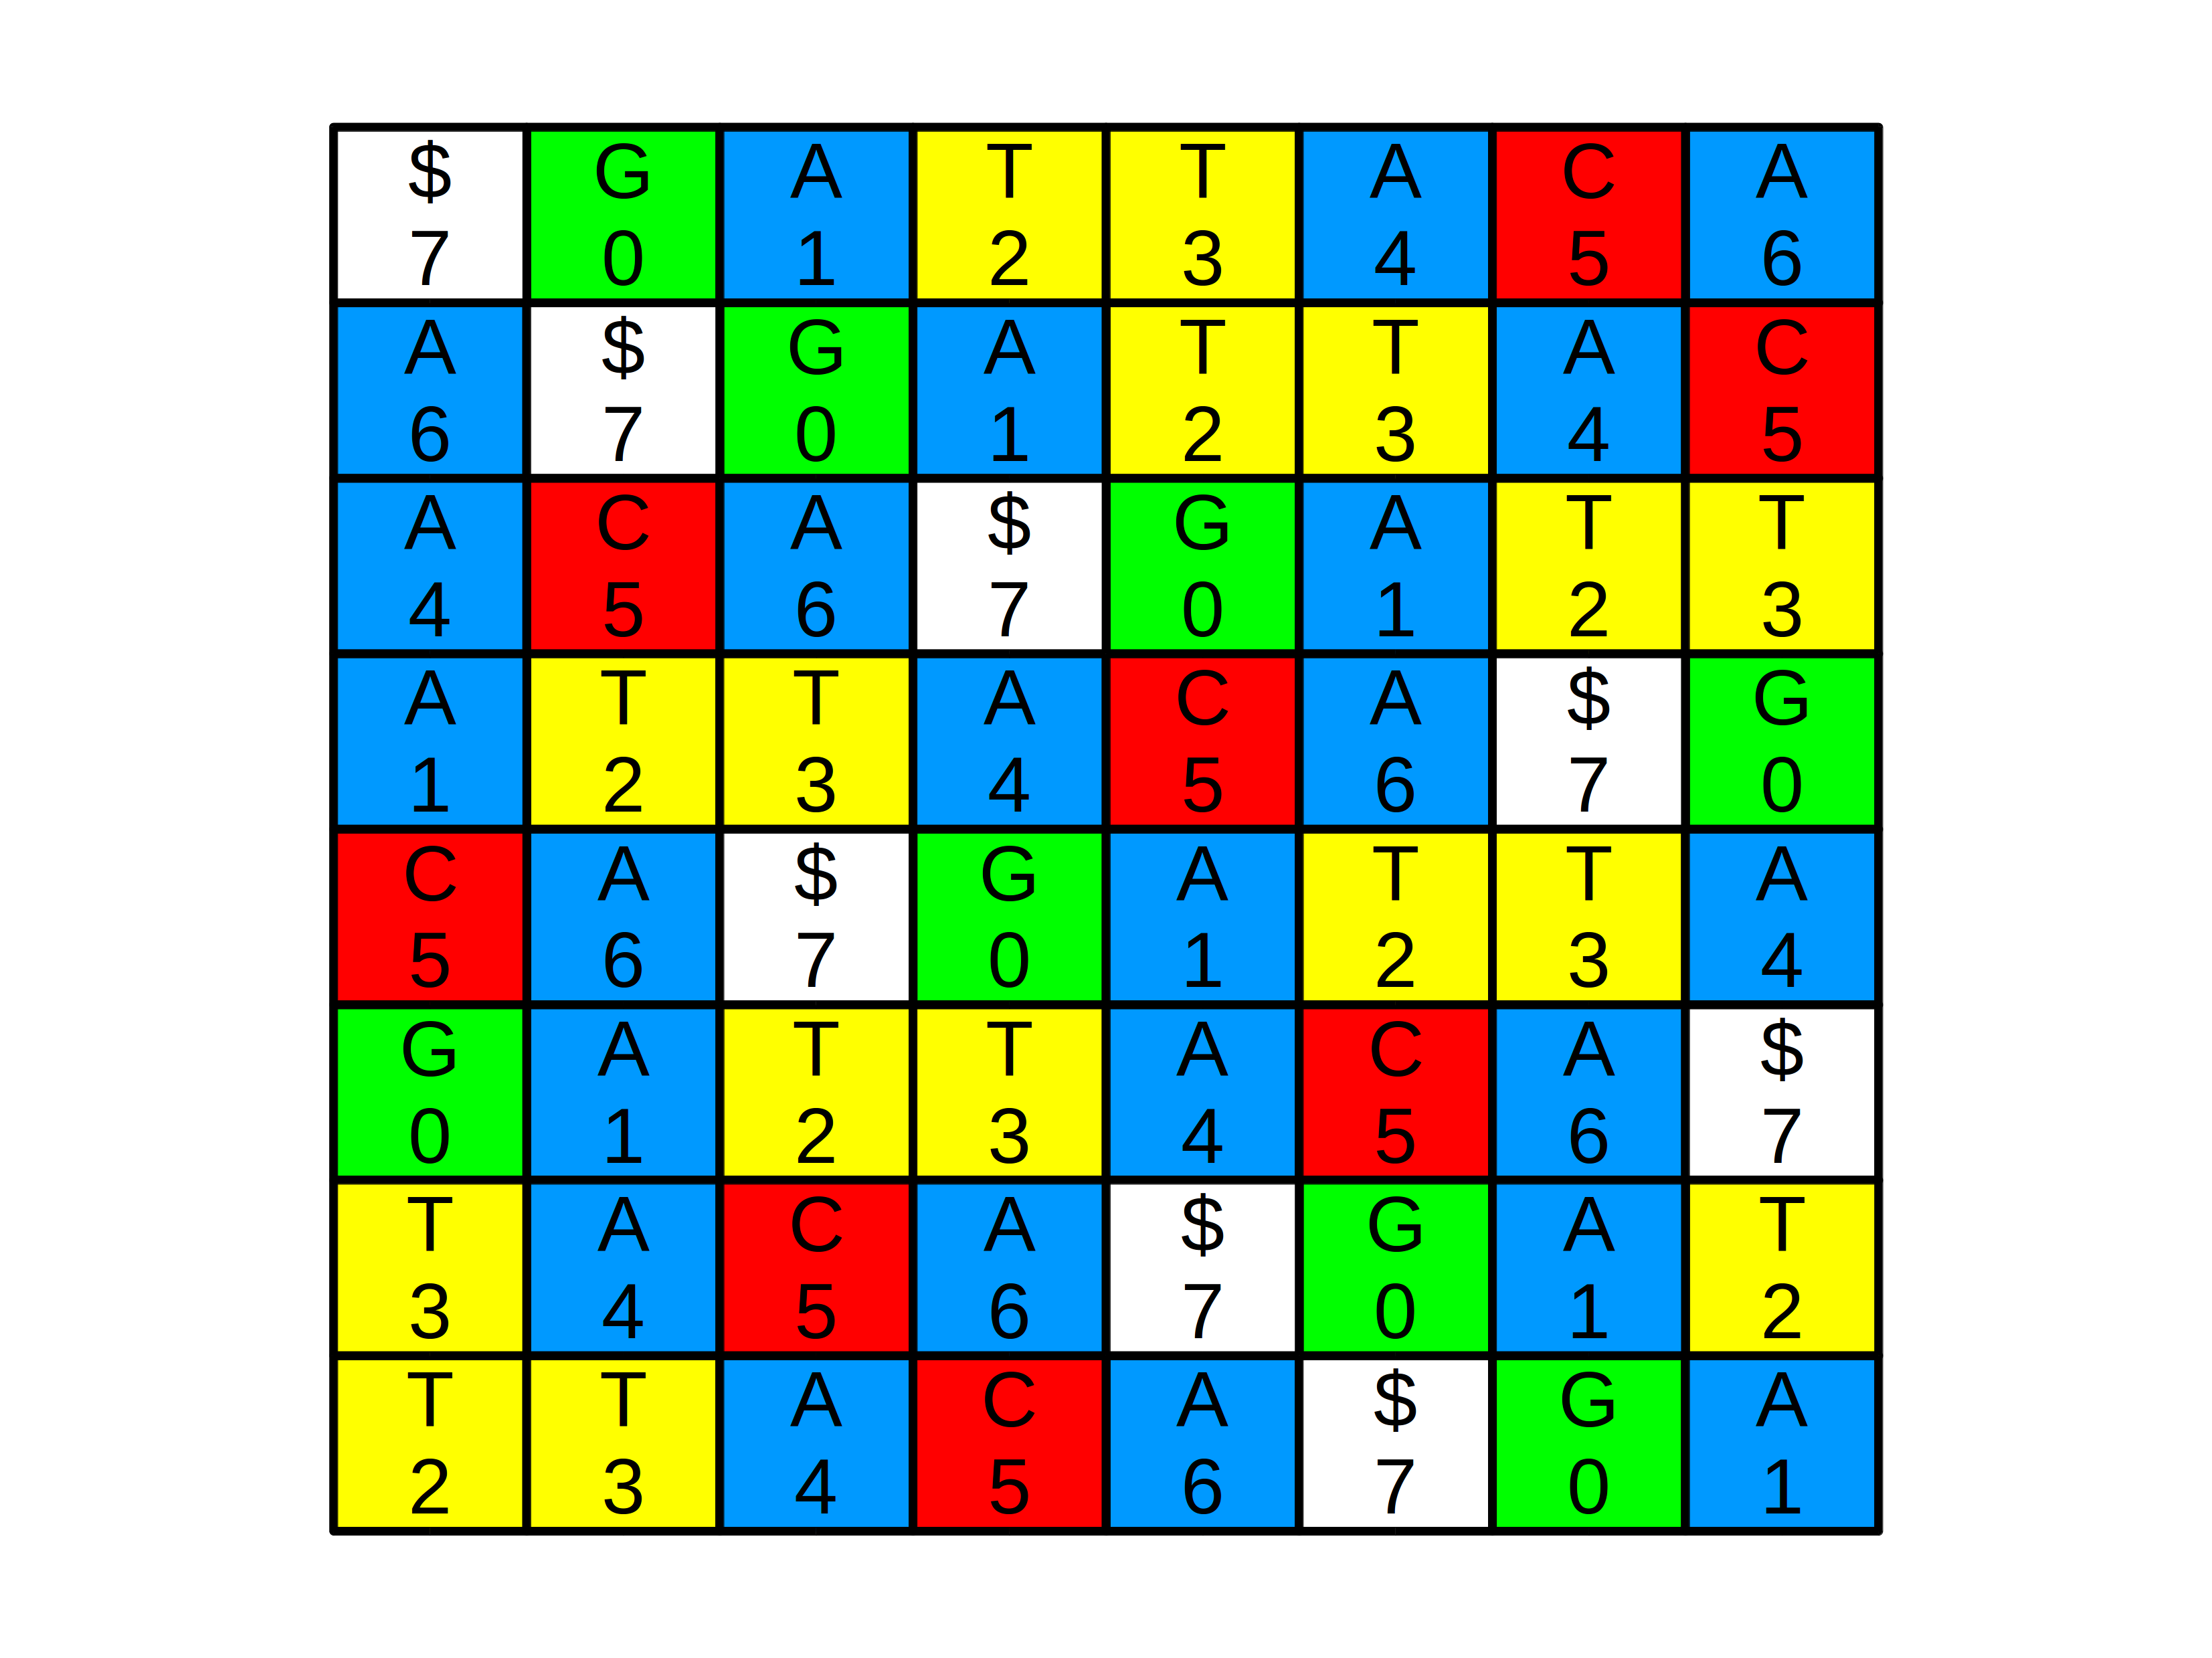
\includegraphics[width=1.0\textwidth]{figures/bwt.png}
    \caption[An example BWT matrix for the string ``GATTACA'']{An example BWT matrix for the string ``GATTACA''. The sentinel value ``\$'' is appended to the end of the string, all rotations of the string are calculated, and the rotations are sorted. Bases are colored according to base identity and numbered according to position in the original string. The characters in the far right column are the BWT of the original string, while the numbers in the far left column are the suffix array (represented as indices into the original string).}
    \label{fig:bwt}
\end{figure}

Note that the instances of any given character in the last column appear in the same relative order in the first column. Consider just the rows where the character in question appears in the first column. When sorting these rows, the first column is uninformative (since it is constant across all rows), and the rows are sorted lexicographically by the remaining columns in order. Rotating all the strings so the uninformative column appears last will not change the order of the other columns, and thus will not change the relative sort order of the rows we are considering. Thus the instances of the character stay in the same relative order in the last column as in the first column \cite{langmead2013introduction}.

% What the BWT is

% How the BWT works
    
    % Imagine all the rotations of the string
    
    % Sort them
    
    % Take the last column
    
\section{Substring Search with the Suffix Array}

The \vocab{suffix array} of a string is an array of indices into the string, sorted in the lexicographical order of the suffixes that they point to \cite{manber1993suffix}. For example, the string ``dog'' has suffixes ``dog'' at index 0, ``og'' at index 1, and ``g'' at index 2, so its suffix array would be $[0, 2, 1]$, corresponding to the suffix sort order $[\textrm{``dog''}, \textrm{``g''}, \textrm{``og''}]$. Another example suffix array is visible in the leftmost column of Figure~\ref{fig:bwt}.

Suffix arrays have some useful properties. Most importantly, all of the suffixes that start with the same substring appear in a single contiguous block \cite{ferragina2000opportunistic}. This block starts at the position corresponding to the number of occurrences of lexicographically smaller substrings of the same length \cite{ferragina2000opportunistic}. This is particularly obvious in the case of single-character substrings: all the suffixes (and, thus, all the substrings) beginning with a certain character appear in one block, coming immediately after all suffixes beginning with lexicographically smaller characters.

Suffix arrays can be used as indices to speed up substring search on the string they are derived from. Because of the block structure described above, and because every instance of a substring is at the beginning of some suffix, a simple binary search is sufficient to find any substring that is present, and a scanning up and down from one instance can pull out the entire corresponding block \cite{manber1993suffix}. Supplementing the suffix array with a \vocab{longest common prefix (LCP)} array, holding the length of the prefix shared by each pair of adjacent suffixes, can further speed up the search, by requiring only a single-character comparison (instead of a string comparison) at each search step \cite{manber1993suffix}.

% What a suffix array is

% Why you can use it for search

% Useful properties
    
    % All the suffixes starting with the same substring are in a contiguous block
    
    % Specifically, all the substrings starting with the same letter are in a contiguous block, which starts at a predictable position based on how many of each character exist in the string.
    
\section{Searching in BWTs with the FM-index}

Constructing the BWT matrix is essentially the same task as constructing the suffix array of the string being transformed. All the rotations of the string contain the ``\$'' sentinel which is lexicographically less than all other characters. Thus the rotations are actually sorted by the portion before the ``\$'' character---that is, by the corresponding suffixes of the original string. This is the same sort used to construct the suffix array.

% OK I can't really connect this to the suffix array properly, but here's how I actually understand it.

A BWT can be augmented with a small amount of additional information to create an FM-index (named after its inventors), which, like a suffix array, allows efficient substring search on the original string, but which also retains the compression afforded by the BWT \cite{ferragina2000opportunistic}. The FM-index is based primarily on the idea of an LF (i.e. last-first) mapping. This mapping maps each character instance in the last column of the BWT matrix to the row in which that same character instance appears in the first column. Because each BWT matrix row is a rotation of the original string, the last column of the row will contain the character instance immediately preceding the one just looked up. Thus, following the LF-mapping around the BWT from any starting position allows the characters of the original string to be enumerated from there in reverse order \cite{ferragina2000opportunistic}.

Since only the last column of the BWT matrix (i.e. the actual BWT string) is used in the algorithm, only that string needs to be stored. Furthermore, the LF-mapping can easily be calculated from the BWT string. To LF-map the character instance at a certain index in the BWT, count up the number of characters in the BWT lexicographically less than the character, and add the character instance's rank among all instances of that character. This gives the index of the LF-mapping result in the BWT.

To see why this works, recall that in a suffix array, and thus also in the BWT matrix, all the suffixes (or here rotations) that start with a given character form a contiguous block, coming just after all those beginning with smaller characters. Thus, the first calculation is to find the start of this block. And since, as shown in Section~\ref{sec:bwt}, the relative order of character instances in the first column is the same as that in the last column, to find the offset of this particular character instance in that contiguous block, we merely need to find its rank among instances of the same character in the last column, which is the BWT string \cite{langmead2013introduction}.

We can now define \vocab{backward search}, a search algorithm using the BWT which processes the characters in the query string from back to front. The algorithm begins by selecting the entire BWT matrix, which is the range of suffixes that begin with the empty string. Then, for each character in the query string, from the last forwards, the algorithm extends the searched string at the front with that character. It takes the new character and finds the first and last instances of it in the BWT contained within the currently selected result range. It then LF-maps each of those instances, and takes the range between them as the new result range for the query string extended with that character. If there are no instances of the character to map, then the searched string is not found in the index \cite{ferragina2000opportunistic}.

Each row of the BWT matrix in the old range started with an instance of the old query string. Each of the rows that ended in the new query character corresponded to an instance of the old query string occurring after the new query character, and thus each implies an instance of the new, one-character-longer query string. The LF-mapping step finds the contiguous block of rows in the BWT matrix where those instances of the search string appear, the boundaries of which correspond to the first and last instances of the new character in the old BWT range (by the conservation of ordering mentioned at the end of Section~\ref{sec:bwt}). Thus, such an algorithm can be used to search for substrings in a string, using the BWT of the string \cite{ferragina2000opportunistic}.

By pre-calculating some auxiliary data structures, such as a table with the start index of each character's range in the BWT matrix, and by using succinct data structures for $O(1)$ rank queries, this algorithm can be made to run in time linear in the length of the query string, and constant in the length of the index \cite{ferragina2000opportunistic}. Furthermore, using a downsampled copy of the suffix array, the location of each result in its source string can be calculated efficiently \cite{siren2009run}.

% TODO: Indexing multiple strings, locate, sampled suffix arrays.

% BWT as an index
    
    % Based on a different way to reverse the BWT using an LF mapping.
    
        % LF mapping goes from a position in the BWT to the position of the character instance that precedes it.
    
    % Sort by context
    
    % FM-index and how it works
        
        % Basically, you are using the BWT and the occurrences to imply the suffix array, and then doing a search on that suffix array.
        
        % Specifically, you have this occurrences array, and this counts array, and follow this formula to shrink a range down to just the range that actually matches your query string.

\section{Bidirectional DNA Search with the FMD-Index}

BWT-based indices have found many applications in genomics, mostly due to their ability to efficiently search for and identify the locations of a substrings in very large data sets---with a few modifications, this search can be extended to align reads to a reference \cite{li2014bwa}. The popular short read aligner \texttt{bwa}, for example, is built on an FM-index of the reference genome; indeed, the name stands for ``Burrows--Wheeler Aligner'' \cite{li2014bwa,li2009fast}. The ``String Graph Assembler'' \texttt{sga} also uses a BWT-based index to do its work, but in this case indexes reads themselves \cite{simpson2012efficient}.

In genomics, the strings being indexed are DNA strings, consisting of As, Gs, Cs, and Ts. These DNA strings are usually excerpts from double-stranded DNA genomes, in which, for each chromosome, two strands of DNA form a double helix. One strand runs in one direction, and the other strand runs in the other direction, with bases complemented (As and Ts swapped, and Gs and Cs swapped). It's impossible to tell whether a DNA sequencing read came from the forward strand or the reverse-complement strand until a match is found for it in a reference somewhere. Thus, many analysis problems in genomics need to consider not only some set of DNA strings but also their reverse complements.

The existence of reverse complements is accounted for in \texttt{sga} by creating two FM-indices of the input data: one index of the forward strand, and one of the reverse-complement strand \cite{simpson2012efficient}. This construction requires DNA query strings to be searched against both indices, and the results combined. However, there is a more elegant approach which allows the same search to be performed against a single index, and moreover allows bidirectional extension of the query string. This data structure, the ``FMD-index'' (the ``D'' is for ``DNA''), is simply an FM-index of both the forward and reverse strands of all input sequences, concatenated into a single data set \cite{li2012exploring}.

The FMD-index provides for double-ended search; that is, an intermediate search result can be extended with a character on either the left or right end of the query string. This works by having the FMD-index store as its intermediate result not just the single range in the BWT corresponding to BWT matrix rows that start with the query string, but also the (equally long) range for the reverse complement of the query string \cite{li2012exploring}. The first is the \vocab{forward range} and the second the \vocab{reverse range}. The fact that these two intervals will always be equally long is the key to the algorithm: because each string in the index is present as both itself and its reverse complement, any appearance of the query string has a corresponding appearance of its reverse complement. Extending the query string on the left causes the forward range to jump around in BWT coordinate space (to the regions of the BWT matrix that begin with the newly added character). However, extending on the left always causes the reverse range to cover a subrange of what it covered previously: the reverse complement of the query string gets extended on the right, and only BWT matrix rows which began with the original reverse-complement query string can possibly also begin with the longer reverse-complement query string.

The FMD-index search algorithm works as follows: When the query string is extended on the left, the forward range is updated as normal. The reverse range takes on the new interval length derived from the forward range, and a small dynamic programming problem is done over the alphabet to find its new start position. The dynamic programming problem is fairly simple because the reverse range can be partitioned into the ranges that would be selected upon left-extension with any character, ordered in lexicographic order by the reverse complement of the character. The dynamic programming simply consists of looping through the alphabet in lexicographic order by reverse complement, considering extending on each character up to the one actually being used, calculating how long the result set would be on the forward strand, and adding that in to the start of the reverse strand interval \cite{li2012exploring}. To extend a string on the right, the forward and reverse ranges are temporarily swapped, and the reverse complement of the query string is extended on its left with the reverse complement of the new base \cite{li2012exploring}.

% TODO: Nobody will possibly be able to understand this. I wish someone else had ever explained this so I could steal their logic. Maybe I need an actual diagram here.

% How the BWT is useful for genomics

    % How some BWT implementations (like RLCSA) fall over when you try and put many gigabytes of stuff in them.

    % And how SGA has a decent implementation of it

% How the FMD-index works

\section{Previous Graph Indices}

The work that I am proposing involves implementing efficient search over graphs of genomic sequence data. This is not a new idea. Many of the current approaches to this problem come at it from the perspective of trying to index a multiple sequence alignment \cite{siren2014indexing}. Two such approaches are described below.

One approach, the Generalized Compressed Suffix Array (GCSA), extends the XBW transform (itself a generalization of the BWT to trees) to ``prefix-range-sorted automata'', which include de Bruijn graphs but not general directed labeled graphs \cite{siren2014indexing}. However, the authors of that approach present only an implementation for acyclic multiple sequence alignments. The existence of nonlinear structures like polymorphic inversions, where a genomic region is forwards in some individuals but backwards in others, is not addressed, and no implementation for de Bruijn graphs is provided \cite{siren2014indexing}. Moreover, the approach presented there provides search over all possible paths through the graph in question, which is a reasonable choice for indices derived from multiple alignments, but which might backfire for graphs with short cyclic structures that could provide pathological productions for many query strings \cite{siren2014indexing}.

Another, slightly newer approach uses the concept of a ``population reference graph'', also derived from a multiple sequence alignment \cite{dilthey2014improved}. In contrast to the BWT-based indexing methods described above, the population reference graph method turns its graph representation of genomes into a Hidden Markov Model (HMM), and identifies the most likely paths through it to match the k-mer spectrum of any particular sample \cite{dilthey2014improved}. Under this method, a pair of haploid genomes are then synthesized as sample-specific references, and existing read-to-genome mapping tools are used to map sequencing reads to these references \cite{dilthey2014improved}. Unfortunately, because of the way that k-mer counts from a sample are divided up to provide input for the HMM model in different genomic regions, this method is forced to divide its HMM states into ``levels'' that it proceeds through in a fixed, sequential order. The resulting graph model is constrained to closely resemble the multiple sequence alignment it was derived from. While this method can effectively model a wide range of alternative sequences in a region, it does not appear to be able to effectively model inversions, duplications, or other more complex structures \cite{dilthey2014improved}.
    
% Talk about that thing that the RLCSA people did that works only for properly sortable graphs or whatever

% Talk about lockstep HMM chromotype approach

    % Not really an index




% We think we can make a better way using a few key technologies

    % We want to make a graph reference
        
        % We already have haplotypes bubbling off, so we really have a graph already
        
        % Benedict did all this previous work on graph genomes
        
    % We want to put this in an aligned hierarchy
        
        % Like something out of HAL, but with a different interpretation.
    
    % We want to employ FMD-index technology and succinct data structures to map to it uniquely at any given level
    
    % We want to employ Spark/GraphX to build a system to traverse and query these graphs
    
    % We want to employ Avro to give this system a consistent API accessible from a variety of languages.

\chapter{Preliminary Work}

I have already completed several smaller projects which are relevant to the work proposed here. The first of these is a web-based tool for visualizing information on cancer patients, which is tied to the project at hand by the thread of spatial metaphors. The second previous project, an analysis of copy number variation in the NOTCH2NL gene family, is an early example of how graphical models accounting for the existence of paralogs can produce useful biological results. The third project, a theoretical treatment of mapping to a graph-based reference genome, lays out a mathematical formalism for some of the problems the current work aims to solve. These pieces of preliminary work illustrate both the need for the current proposed research and my competence to carry it out.

% I have already some some work on infrastructure for the scalable analysis of genomic variation.

\section{Project \#1: Tumor Map Visualization}

The first piece of preliminary work presented here is the UCSC Tumor Map, visible in Figure~\ref{fig:tumormap}. The Tumor Map is a web-based interactive analysis tool for exploring cancer data sets. I developed the first version of the tool for a quarter-long rotation project in the Stuart Lab here at UCSC, and I have since been working with others in that lab to add new analysis features and to polish the tool for publication.

\begin{figure}[ht]
    \centering
    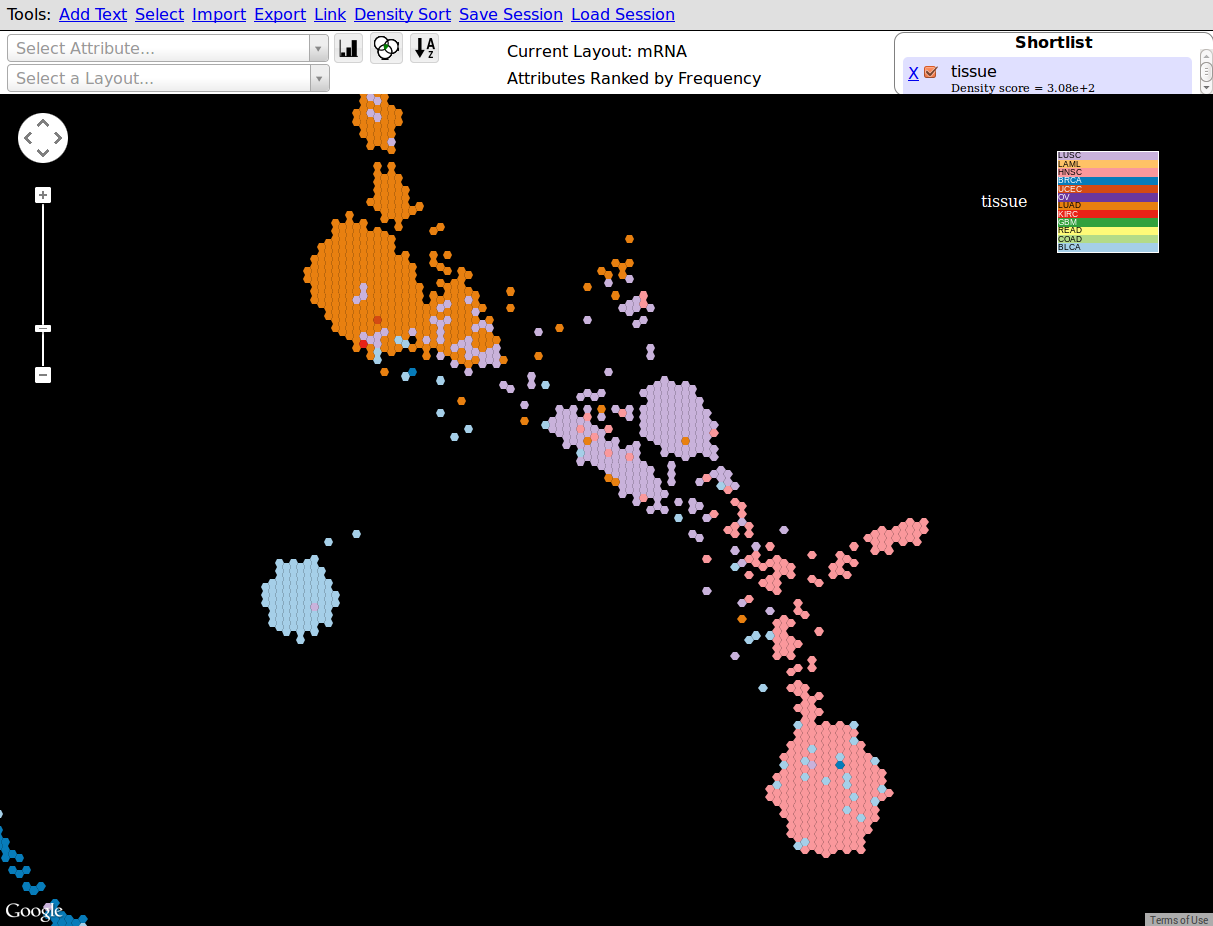
\includegraphics[width=1.0\textwidth]{figures/tumormap.png}
    \caption[A screenshot of the UCSC Tumor Map]{A screenshot of the UCSC Tumor Map. Individual tumor samples are represented by hexes in a hexagonal grid, laid out using a spring layout algorithm based on molecular similarity. The map is browseable using a Google Maps interface. Hexes can be colored using various data overlays, and statistical queries can be run interactively.}
    \label{fig:tumormap}
\end{figure}

The visualization itself consists of a hexagonal grid on which tumor samples are arranged, with at most one sample in each hex. Samples are arranged according to sample-sample similarity values from a similarity matrix, which are then used as spring strengths in the DrL graph spring layout algorithm \cite{martin2008drl}. Spring layout positions are then discretized on a hexagonal grid. If the hex a sample would occupy is already filled, it is placed in a minimally distant free hex. This algorithm is found to produce ``islands'' of similar samples, with some interaction between and substructure within them \cite{novak2014ucsc}.

The hexagonal grid is conceptually a map: tumor samples are placed close to relatively similar samples, and far from relatively different ones. This creates a two-dimensional space in which scientists can form and test hypotheses about what features drive these similarities and differences. To aid in this process, the Tumor Map provides a facility for displaying attribute overlays, allowing continuous, binary, or categorical per-sample data to be visualized in this space. By default, the visualization displays a tissue overlay, coloring each sample according to the tissue from which the tumor was originally derived. Other attribute overlays, like mutations in important cancer genes, or the relative levels of activation of various transcriptional programs, can be brought up using the dropdown in the upper left. Up to two can be displayed at a time, using a dynamically-generated combined color scheme.

The visualization provides facilities for running statistical tests on the attribute overlays. When the visualization is first opened, attributes are sorted by a layout-aware density metric. Attributes whose high or low values are significantly clustered together in the space defined by the map being sort to the top of the list. Other available statistical tests include layout-aware and layout-independent association tests, for finding other attributes statistically significantly related to a ``pivot'' attribute, and a dichotomy-based sort, for finding attributes that are statistically significantly different between two user-selected groups of samples. Using these tools, scientists can quickly ask and answer questions like ``what's special about this little clump of tumors budding off from this island?'' or ``what other mutations show up near TP53-mutated tumors in this space?''.

The current official Tumor Map visualization is built against the TCGA PanCancer data set, with a variety of locally-produced and imported overlays. However, I implemented the generator as a Galaxy tool, so it can be used to generate a visualization from any appropriately formatted similarity matrix and set of overlays \cite{weinstein2013cancer,giardine2005galaxy}. The full details about the data that went into the current sample visualization, as well as more information on the algorithms used, can be found in \cite{novak2014ucsc}.

The UCSC Tumor Map is worth mentioning here primarily because it illustrates my ability to execute large tool-building projects. It is also an object lesson in the importance of spatial metaphors, especially important when I am proposing to change the space in which human genomics is practiced. The Tumor Map's primary focus is bringing the concept of space to pan-cancer tumor analysis, and, judging by other scientists' reactions to the tool, it is clear that scientists value the use of spatial thinking to understand datasets. I will apply this lesson on the importance of spatial metaphors to the development of the graph-based reference representation I propose here.

% I made a pan-cancer visualization of the entire cross-tissue TCGA data set
    
    % Lay out all the tumors by a similarity metric, and squish them into a hexagonal grid in 2D
    
    % Let people fly around it with Google Maps
    
    % Then draw map overlays depicting various tumor or patient attributes.

    % Less a scaling up of the analysis than a scaling down of the data set into a space where people are comfortable working.
    
% See the paper. 

\section{Project \#2: NOTCH2NL Copy Number Variation Analysis}

My graph-based analysis of NOTCH2NL paralog copy number is a second and somewhat more relevant piece of prior work. As discussed in Section~\ref{sec:notch}, while the older GRCh37 human genome assembly had only a single NOTCH2NL gene annotated, new information from sequencing haploid cells (from a hyatidiform mole) revealed the existence of four paralogs, here dubbed NOTCH2NL-A, NOTCH2NL-B, NOTCH2NL-C, and NOTCH2NL-D \cite{jacobs2014recently}. Moreover, NOTCH2NL-A, -B, and -C were found to be located quite close to ``the 1q21.1 distal deletion/duplication locus'' \cite{jacobs2014recently}, copy number variations of which have been associated with congenital microcephaly and macrocephaly \cite{jacobs2014recently}. The goal of our project was to determine if deletions or duplications of any of the nearby NOTCH2NL genes could potentially explain these microcephalic and macrocephalic phenotypes.

Our lab took several approaches to answering this question, including experimental wet-lab characterization of the NOTCH2NL proteins' effects on mice and reanalysis of high-throughput-sequencing data to look at copy number variations in these genes in the general population \cite{jacobs2014recently}. The approach that I took, however, relied on a collection of DNA microarrays from people with microcephaly, people with macrocephaly, and people with neither condition \cite{jacobs2014recently}.

The microarrays I used provided comparative genomic hybridization (CGH) data: for each probe, the array gave what was supposed to be the ratio of the amount of matching DNA in the sample to the amount of matching DNA in a standard ``normal'' genome that was also hybridized to the array. As microarrays were involved, so was a tedious amount of normalization, which is described in full in the supplement of \cite{jacobs2014recently}. Briefly, my analysis pipeline worked by first re-mapping the sequences of the microarray probes to the hyatidiform mole assembly with pblat, and taking all hits \cite{meng2012parallelized}. Probes that had no mapping locations near the region of interest were ignored. The relative affinity of each probe for hybridizing with each of its mapping locations was calculated using DECIPHER \cite{wright2012decipher}.

This information on probe mapping locations was used to create an integer linear programming (ILP) model of the sample and standard normal genomes. Such a model can be thought of as a graph of variables connected by linekar constraint hyperedges. Each probe mapping location became two graph nodes, one representing its copy number in the sample, and one representing its copy number in the standard normal genome (which may have itself had copy number differences relative to the hyatidiform mole assembly). Each mapping location in each genome had a linear programming variable representing its copy number, and constraints were added penalizing copy number differences between adjacent probe mapping locations. For each probe, all of its mapping locations in each genome were linked together in an affinity-weighted sum representing the total hybridization of that probe in that genome; the hybridization levels of each probe in each genome were constrained together to penalize deviation from the observed microarray hybridization ratios for the sample being analyzed (after normalizing against a series of control samples for the array, if available). Additionally, all copy number estimates were slightly penalized for deviations from the ordinarily expected value of 2 copies, which is a fairly strong prior on copy number in a diploid genome. Each sample's linear programming problem was solved with the CBC linear programming solver, finding optimal copy numbers for each probe mapping location in each genome under the constraints \cite{forrest2013cbc}. The process was repeated with different linear programming objective penalty weights in order to distinguish high- and low-confidence copy number changes.

\begin{figure}[h!t]
    \centering
    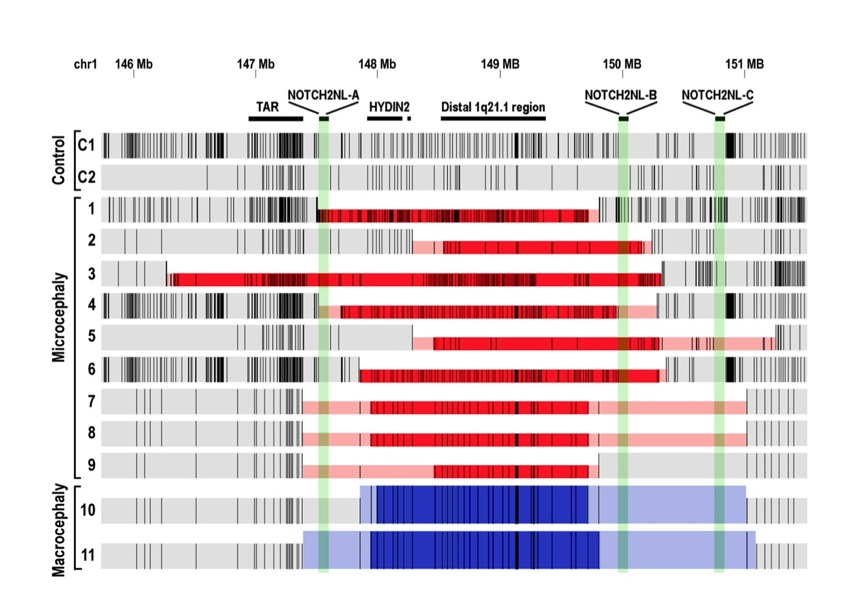
\includegraphics[width=1.0\textwidth]{figures/notch2nl.png}
    \caption[Results from the linear programming copy number inference pipeline]{Results from the linear programming copy number inference pipeline. Patients with microcephaly have red highlights, patients with macrocephaly have blue highlights, and control patients have no highlights. Regions which are potentially (light) or with high confidence (dark) altered in copy number are highlighted. Black lines show linear-programming-processed copy numbers at microarray probe binding locations. NOTCH2NL-B copy number is reduced with high confidence in 4 of 8 patients with microcephaly. NOTCH2NL-A copy number is reduced with high confidence in 2 of 8 patients with microcephaly. The dataset is consistent with at least one copy of NOTCH2NL-A or NOTCH2NL-B being deleted in each microcephaly patient, and at least one being duplicated in each macrocephaly patient. No copy number alterations were detected in any of the NOTCH2NL genes for any of the controls. Adapted from \cite{jacobs2014recently} Figure 5B.}
    \label{fig:notch2nl}
\end{figure}

The results of this process are visible in Figure~\ref{fig:notch2nl}. I found copy number changes in the region of interest in all of the microcephaly and macrocephaly patients examined, and in none of the controls. Moreover, the copy number changes in all microcephaly patients were consistent with a deletion of NOTCH2NL-A or NOTCH2NL-B (or both), and likewise the copy number changes in the two macrocephaly patients were consistent with similar duplications. Unfortunately, the NOTCH2NL genes did not always fall in the regions where copy number was determined to have been altered with high confidence; this only happened in 4 of the 8 microcephaly patients, and neither of the macrocephaly patients. However, this is in part due to the sparsity of probe mapping locations in the vicinities of the NOTCH2NL genes, where the hyatidiform mole assembly provides novel sequence which the probes were not designed to target.

This prior work serves the project being proposed now as an illustration of the usefulness of graphical models of genomes and of genomic variation. The use of a graphical model here allowed information to be extracted from microarray probes which did not unambiguously map to the reference genome used. This in turn allowed data from microarrays designed with an older reference to be effectively used with our new custom assembly. Furthermore, several seemingly distinct structural variants were uncovered in the region examined here. Although I hypothesize them to be private to the individuals in this study, it is clear that, if one wanted to store them in some sort of database of variation, one would need a way to effectively represent several partially overlapping structural variants---a task for which graph representations are well-suited and VCF is not.



% I made a first pass at analyzing the NOTCH2NL region
    
    % I specifically worked on a linear programming based approach to make copy number calls on our corrected assembly using CGH microarray probes originally designed for an assembly that conflated the NOTCH2NL genes
    
    % Trying to handle multimapping, because if I threw out multimapping I would have thrown out XX% of the data.
        
        % This again isn't really scaling, but it's something we need to do to support scaling.
    
% We found that CNV in the NOTCH2NL region can explain disease.

    % See the paper.

\section{Project \#3: Mapping to a Reference Genome Structure}
\label{sec:mapping}

In order to implement any sort of new data structure, it is necessary to work out what operations the structure is to support and what algorithms can provide them. To that end, as a preliminary to the work proposed here, we have developed a rigorous mathematical model of ``reference structures'' and their associated operations \cite{paten2014mapping}. My contribution here was primarily as a tester of the theory, contributing counterexamples and demonstrations of impracticality to make our current model stronger. Long portions of the following description of that model are adapted from \cite{paten2014mapping}. 

% TODO: This section is lifted from the paper and needs to fit in with the rest (i.e. match in person and stuff).

% TODO: Make this section explanatory so you can understand where we're going with this.

We model both reference and individual genome assemblies as \vocab{sequence graphs}, which allow for a more general class of assembly representation, and which incorporate phased contig/scaffold representations as a special case. 

A \vocab{base instance} is a pair $(b,P)$ consisting of a labeling base $b$ in $\{\mathrm{A},\mathrm{C},\mathrm{T},\mathrm{G}\}$ and a \vocab{position} $P$. All positions are globally unique, so given a position $P$, one may determine the base at that position, i.e. the unique $b$ such that $(b,P)$ is a base instance. The nucleotides in all genomes are described as base instances. 

In order to define a sequence graph, we need to specify how base instances are connected to form sequences. To do this generally, as DNA is double stranded, we must distinguish the forward and reverse complement orientations of base instances. Each base instance $(b,P)$ has a \vocab{left side}, denoted $P_l$, and a \vocab{right side}, denoted $P_r$. An \vocab{adjacency} is an unordered pair of two sides; an adjacency ${P_s, Q_t}$ asserts that the $s$ side of the base at position $P$ is connected to the $t$ side of the base at position $Q$. 

A \vocab{sequence graph} $G = (V_G,E_G)$ is a bidirected graph \cite{medvedev2009maximum} in which each node in the set $V_G$ of nodes is a base instance and each edge in the set $E_G$ of edges is an adjacency connecting the sides of two base instances. The forward label of a node $(b,P)$ is the base $b$, and the reverse label is the reverse complement base $b^*$, where $\mathrm{A}^* = \mathrm{T}$, $\mathrm{T}^* = \mathrm{A}$, $\mathrm{G}^* = \mathrm{C}$, and $\mathrm{C}^* = \mathrm{G}$. Using its sides for orientation, for a base instance $(b, P)$ we write $b(P_l) = b$ and $b(P_r) = b^*$ to denote the base label oriented by the given side.

A \vocab{linear thread} is a special kind of path in a sequence graph composed of a sequence of oriented nodes and edges between them, such that each node other than the first and last node on the path is entered on one side and exited on the other. Nodes can be visited more than once in a thread. The \vocab{traversal} of a thread specifies a sequence of nucleotides, decoded by enumerating the labels of base instances in the order and orientation specified by the thread, such that if a base instance $(b, P)$ is oriented from $P_l$ to $P_r$ then $b(P_l) = b$ is incorporated into the traversal, and if oriented from $P_r$ to $P_l$ then $b(P_r) = b^*$ is incorporated into the traversal. A \vocab{circular thread} is a circular path of oriented nodes and edges in which each node is entered on one side and exited on the other. Its traversal is a circular sequence of nucleotides, similar to mitochondrial or bacterial sequences.  

A \vocab{contig graph}, or \vocab{contig}, is a sequence graph that consists of a single linear or circular thread with no node repetitions. A \vocab{phased} sequence graph is a sequence graph consisting of a set of disjoint contig subgraphs.

Any sequence graph that is not a phased sequence graph is called \vocab{unphased}. Unphased sequence graphs can be used to represent genomes in which there is some uncertainty in phasing or assembly. They can also be used to represent populations of genomes in which numerous variations are described, e.g. an extension of a reference genome assembly to include more than one variant of some regions

Let us assume that we are given an input sequence graph $G$ and a target sequence graph $H$. The task is to map the input base instances in $V_G$ to corresponding target base instances in $V_H$. Often the input graph will represent the genome of a particular individual and the target graph will be used as a reference genome. To avoid wrongly categorizing genetic variations in the input graph, we leave a base instance in $V_G$ unmapped if it can plausibly map to more than one base instance in $V_H$. The mapping may therefore be partial; i.e. it is not assumed that all elements of VG will be mapped. Since the identifier $P$ of the base instance $(b,P)$ determines the base $b$, it suffices to map positions uniquely to positions, i.e. identifiers to identifiers. However, to account for the double-sided nature of DNA strands, we must allow a position $P$ in $G$ to map to a position in $H$ in either the forward or reverse orientation. Formally, a mapping from a sequence graph $G$ to a sequence graph $H$ is a partial function $M$ from the set of positions in $G$ to the set of positions in $H$ such that for every position $P$ in $G$, either $M(P)$ is undefined and we say that position $P$ is \vocab{unmapped} in $H$, or there is a position $Q$ in $H$ such that $M(P) = Q$ and either $b(P_l) = b(Q_l)$ (and we say that $P$ is \vocab{forward mapped} to $Q$ in $H$), or $b(P_l) = b(Q_r)$ (and we say that $P$ is \vocab{reverse mapped} to $Q$ in $H$). In either of the latter two cases we say that position $P$ \vocab{maps} to the position $Q$ in $H$ (or more generally that the position $P$ is mapped in $H$).  

Let $H$ be a phased sequence graph to be treated as a target (e.g. reference) genome. For each side $Q_s$ in $H$ the \vocab{unique context} of $Q_s$, denoted $U(Q_s)$, is the shortest suffix $u$ of the traversal of a thread in $H$ ending at $Q$ entered from its $s$ side, such that $u$ occurs exactly once as a traversal of a thread in $H$ (ending at any side of any node). The suffix $u$ includes the base of $Q$, and does not always include other bases. If no such unique suffix $u$ exists for $Q_s$, we say that the side $Q_s$ is \vocab{unmappable}.

For a side $P_s$ in a phased sequence graph $G$, $P_s$ is matched to a side $Q_t$ in a phased target sequence graph $H$ if a suffix of the traversal of the thread ending at and including $P$ entered from its $s$ side is the same as $U(Q_t)$. The essential property of the unique contexts of $H$ is that, as a family, they don't share suffixes, which means any side in any $G$ can be matched to at most one side in $H$. 

Given the above matching of sides, the left-right exact match mapping $M_e$ of positions is defined as follows. A position $P$ in $G$ is:
\begin{itemize}
\item \vocab{unmapped} in $H$ (and $M_e(P)$ is undefined) if neither $P_l$ or $P_r$ are matched anywhere, 
\item \vocab{left-mapped} at $M_e(P) = Q$ if $P_l$ is matched to a side of $Q$, but $P_r$ is not matched anywhere, 
\item \vocab{right-mapped} at $M_e(P) = Q$ if $P_r$ is matched to a side of $Q$, but $P_l$ is not matched anywhere,
\item \vocab{fully-mapped} at $M_e(P) = Q$ if $P_l$ is matched to one side of $Q$ and $P_r$ is matched to the other side of $Q$,
\item else $P$ is \vocab{inconsistently-mapped} in $H$ (and $M_e(P)$ is undefined).
\end{itemize}

Combining cases, we say that position $P$ is mapped in $H$ if it is left-mapped, right-mapped or fully-mapped, and not mapped in $H$ if is it either unmapped or inconsistently-mapped. This defines the left-right exact match mapping $M_e$ from $G$ to $H$. 

A \vocab{mapping scheme} for a sequence graph $H$ is a definition, rule or procedure that defines a mapping $M$ from positions in $G$ to positions in $H$ for all possible sequence graphs $G$. The pair $(H, M)$, consisting of a sequence graph $H$ and a mapping scheme for $H$ is called a \vocab{reference structure}. For example, if $H$ is a phased sequence graph and we define the mapping $M$ from $G$ to $H$ to be the mapping $M_e$ for each phased sequence graph $G$, and leave the mapping of every position in a unphased input graph $G$ undefined, then $M$ is a mapping scheme for $H$ and $(H, M)$ is a reference structure. 

A \vocab{reference hierarchy} is a collection of reference structures at different levels, one built upon another. A higher-level reference structure is derived from a lower-level reference structure by merging some base instances in the lower-level structure together, and re-numbering all the nodes in the new structure as new positions. Base instances can only be merged if they share a base (in which case their corresponding sides are combined) or if they have complementary bases (in which case their opposite sides are combined). A \vocab{merging scheme} is an algorithm that specifies what base instances to merge when creating a higher-level reference structure. One example of a merging scheme is the \vocab{$\boldsymbol{p}$-overlap merging scheme}, in which base instances whose contexts on one side match out to at least distance $p$ are merged. (However, see Subsection~\ref{subsec:aim1merging} for issues I uncovered with this na\"{\i}ve scheme.)

Toy examples of reference structures are given in Figures~\ref{fig:lrexactmatch} and~\ref{fig:lrexactmatchgraph}. A full description of reference structure theory is available in \cite{paten2014mapping}.

\begin{figure}[ht]
    \centering
    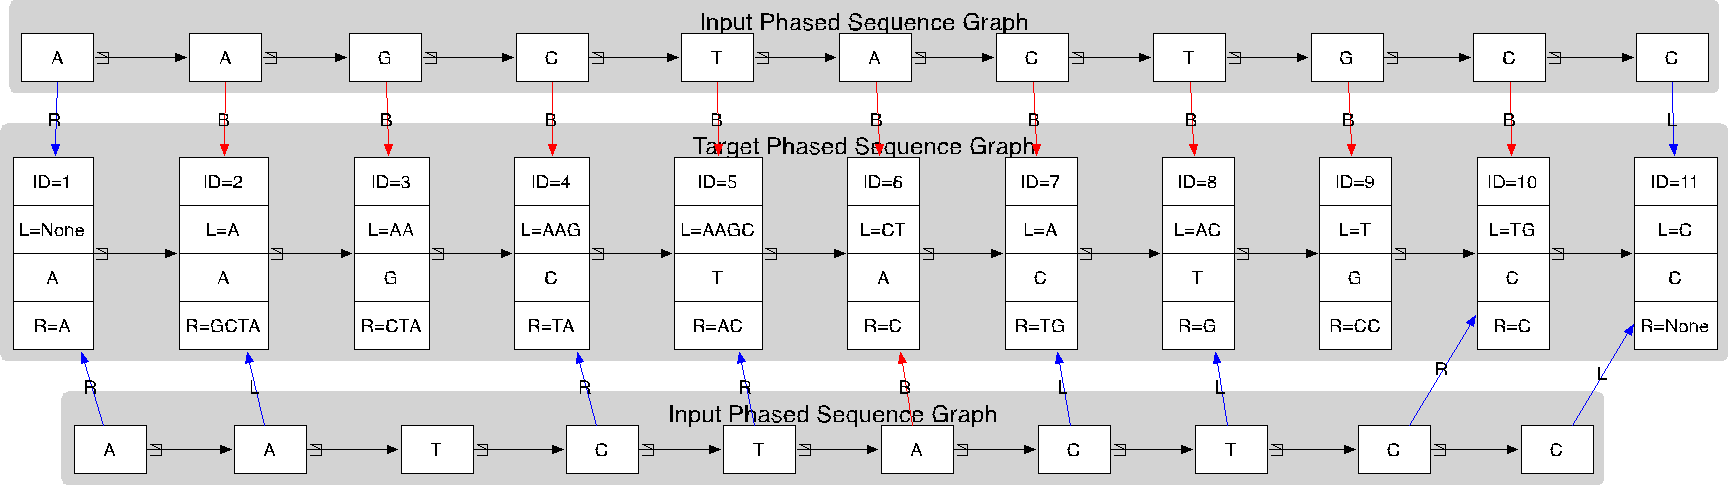
\includegraphics[width=1.0\textwidth]{figures/lrexactmatch.png}
    \caption[An example of reference structure mapping]{An example of reference structure mapping. Two query sequences (top and bottom) are mapped to a left-right exact match reference structure (middle). Shown here are the unique contexts for every side in the sequence graph. For a node $(b, P)$ denoted with $L=t$ and $R=u$ the left unique context is the string $tb$ and the right unique context is the string $(bu)^*$; in this and subsequent figures the right unique context string is shown as its reverse complement so that both unique contexts of a position can be read from left-to-right. A side labeled ``None'' is unmappable. Adapted from \cite{paten2014mapping} Figure 5.}
    \label{fig:lrexactmatch}
\end{figure}

\begin{figure}[ht]
    \centering
    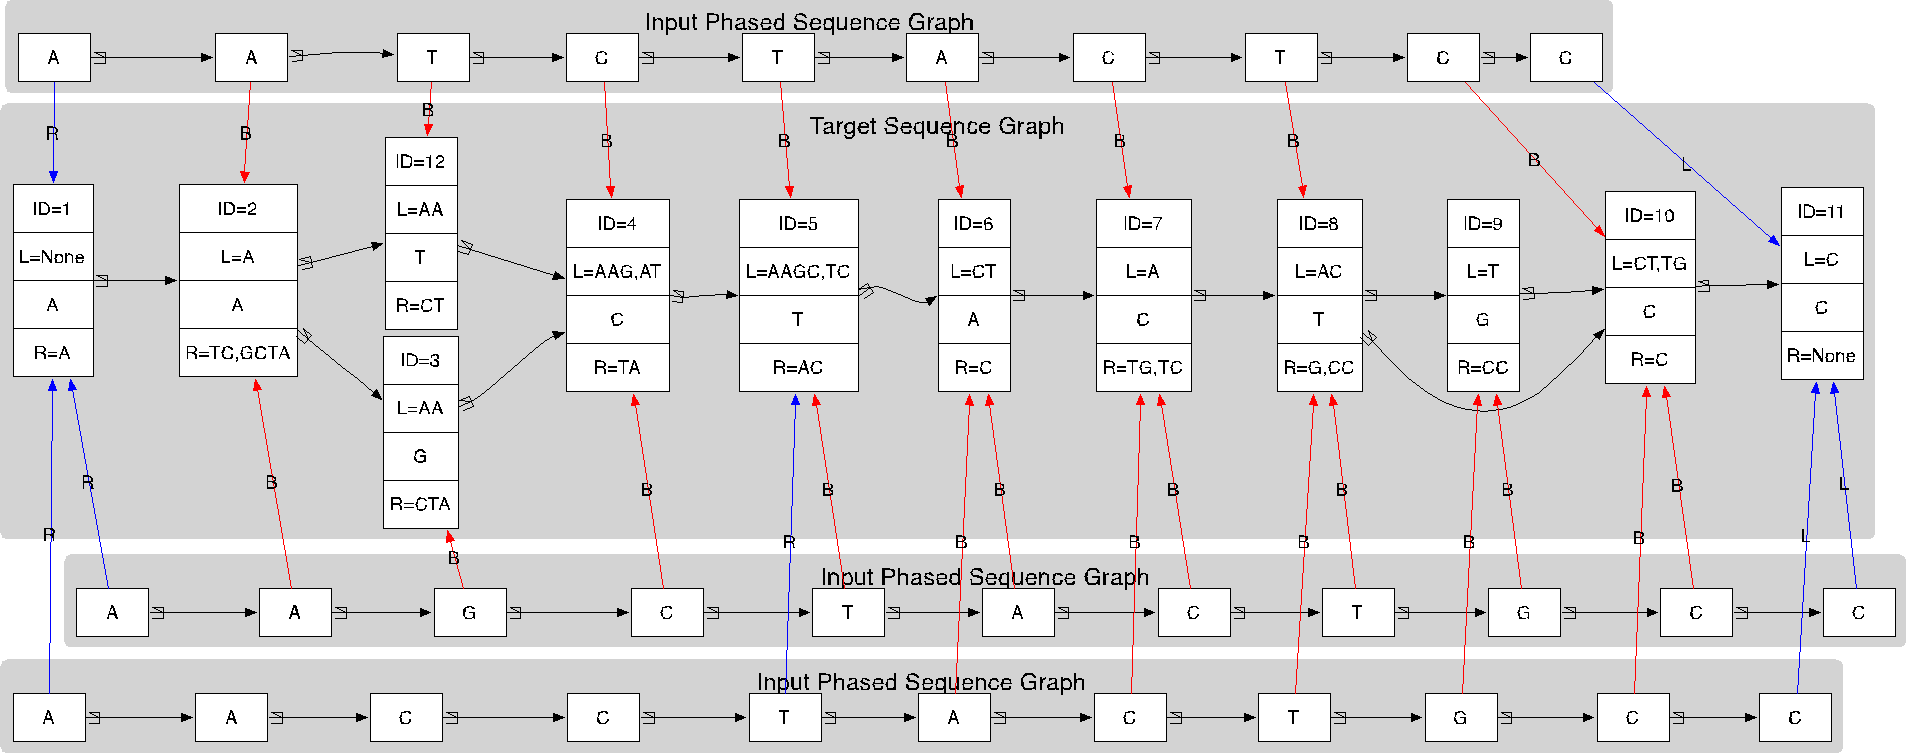
\includegraphics[width=1.0\textwidth]{figures/lrexactmatchgraph.png}
    \caption[An example of left-right exact match mapping]{An example of left-right exact match mapping. Phased input sequence graphs are mapped to a target unphased sequence graph. The two haplotypes used to build the target sequence graph are shown as the input sequence graphs immediately above and below the target sequence graph. L and R are left and right minimally unique contexts for all threads (excluding the base itself). A novel haplotype is shown at the bottom as an input sequence graph mapped to the target sequence graph. Adapted from \cite{paten2014mapping} Figure 6.} 
    \label{fig:lrexactmatchgraph}
\end{figure}

This piece of preliminary work is important to my project because it defines the mathematical framework that I will be working in. Some of the more advanced mathematical models for our very latest mapping and merging schemes need to be finalized, but they are all built on this foundation of a formal description of sequence graphs, reference hierarchies, and the operations on them. Furthermore, my participation in the development and refinement of this mathematical framework illustrates that I understand it and am able to work with it competently---prerequisites for implementing it in software.

% We developed a rigorous theory for making reference graphs, putting them in hierarchies, and mapping to them based on context.

% I'm going to need this in my system as an alternative to linear coordinates, since linear coordinates have all the problems mentioned above.

% The hierarchy stuff is also how I plan to formalize multimapping into something useful.

% See the paper.

\chapter{Proposed Work}

Building on the foundation of the preliminary work described above, I propose a three-part research agenda. First, I will further develop the reference structure theory just described with new mapping and merging schemes, culminating in the publication of a complete paper describing the theory and its new extensions. Second, I will implement this extended theory in a set of scalable software tools, using advanced string and graph indexing algorithms. These tools will present a well-defined API, suitable for use in a shared-infrastructure environment. Finally, I will use these tools to explore human genomic regions which have hitherto frustrated traditional analysis methods, like the major histocompatibility complex, the 1q21.1 region of chromosome 1, and the centromeres, in hopes of discovering and characterizing potentially important structural variation.

\section{Specific Aim \#1: Develop Reference Hierarchy Theory}

The first component of my project is to further develop the formalisms of mapping schemes, reference structures, and reference hierarchies. I will create a system that can replace existing alignment formalisms and traditional ways of conceptualizing the reference genome.

\subsection{Define a Practical Merging Scheme}
\label{subsec:aim1merging}

One of the major tasks here is to come up with formalized, practical merging schemes. The $p$-overlap merging scheme \cite{paten2014mapping}, for example, has turned out to be quite impractical; when applied to real-world MHC data in a prototype implementation, it merges hundreds of thousands of unrelated bases together. I will identify, formalize, and prototype a more practical merging scheme.

The current prototype merging scheme that I have implemented is the \vocab{greedy merging scheme}. It works by starting with a high-quality linear reference sequence (such as the GRCh38 golden path) which is implicitly taken as an initial reference structure. It then takes additional ``genomes'' of linear contigs, and maps them to the reference structure using the mapping scheme. The newly mapped base instances are merged with the base instances that they mapped to, the reference structure is rebuilt, and the process continues with the next genome. 

Although this merging scheme suffers from some theoretical shortcomings---for example, the results are dependent on the order in which genomes are added---in practice qualitatively clean-looking reference structures are produced. Moreover, the positions of the initial reference structure (i.e.\ the GRCh38 primary path) are never merged with each other, making this an attractive merging scheme for creating a reference structure (and associated graph-based coordinate system) which is backwards-compatible with existing GRCh38 linear coordinates. Finally, since the procedure to place new variants in the reference graph is exactly the same as that used to map new samples to the reference graph, this merging scheme provides an obvious update path.

To complete this part of the project, I will need to define a mathematical model of the greedy merging scheme in the language of reference structure theory, and prove its essential properties. I will also need to demonstrate that it is practical to apply it at the scale necessary to complete Specific Aim \#2 (Section~\ref{sec:aim2}), through prototyping.

\subsection{Define a Practical Mapping Scheme}
\label{subsec:aim1mapping}

Hand in hand with the above, I will also need to formally define and test a practical mapping scheme, both for mapping during the construction of a reference structure, and for mapping short reads (and upcoming long reads) to that reference structure. In this area my prior work has proven more fruitful. I have prototyped the (general) left-right exact match mapping scheme of Section~\ref{sec:mapping}. When used with the greedy merging scheme, left-right exact match mapping can produce a reasonable-looking reference structure out of the GRCh38 MHC region and its alt loci. However, that reference structure is still not all that great; there are large regions which are not merged due to mismatches or other small differences between the sequences being merged.

In order to rectify this problem, our lab has been working on alternative methods of mapping. One of the alternatives we are exploring is to post-process mappings from the left-right exact match scheme, automatically identifying ``bubbles'' of sequence which did not map together and trying to ``zip'' them closed by pairing up identical bases. Another student in the lab has looked at this option, which we have termed ``mapping on credit'', prototyped it, and determined that it can be formalized appropriately under our model; I will have to do (or perhaps merely adopt) this formalization.

Another alternative that we are looking at is adding support for a limited number of mismatches. Another student in our lab has also been working on prototyping this, and it seems to be a better mapping scheme in terms of coverage, but also much slower, at least in its current prototype form, than the exact match version. I will need to speed up our prototype of this mapping scheme as much as possible in order to see if it would be practical to apply it on a larger scale.

\subsection{Construct a Mathematics of Variants}
\label{subsec:aim1math}

In addition to fleshing out the mathematical models of reference structures as they relate to mapping, I will also need to define mathematical tools for using reference structures, or perhaps more stripped-down sequence graphs without some of the mapping equipment, as repositories of information about genomic variation. A good reference structure for humans might be expected to include, in addition to the alleles represented by GRCh38 and its alt loci, information about other forms of variation. SNPs, short indels, and structural variants the GRC did not deem worthy of promotion to full alt loci would all appear. Having built this graph of human variation, it would be a poor decision to use it only for mapping and not for variant storage and analysis.

In order to use reference structures as a language for variation, I will need to define a mathematics of variants, with rigorous formal definitions of what variants are, and the operations they support. As a part of this I will also need to formalize a graph representation of partially phased individual genomes, because modeling samples is an important part of modeling variation.

Some work is already being done in this area, and I will strive to be compatible with it. For example, my lab is involved in the Global Alliance for Genomics and Health (GA4GH), an organization which is currently working on a graph-based format for representing variation. This format is based around a concept of variants being unary, as opposed to part of a set of alternative alleles \cite{ga4gh2014variation}. I will adopt and formalize these concepts.

\subsection{Deliverables}
\label{subsec:aim1deliverables}

The culmination of this part of the research program will be a publication detailing the theory needed to build the software tools that come next. I will also deliver prototypes demonstrating that the mathematical formalisms I choose can be practically applied to real data at nontrivial (although not necessarily genomic) scales. These prototypes will in turn be used to compare the empirical performance of formalized reference structure theory merging and mapping to that of other methods of haplotype and read alignment.

% I need a rigorous theory of reference structures, reference hierarchies, mapping, and multimapping

    % We defined one, but it still has some problems
    
    % The p-overlap merging scheme is unworkable. It collapses too much stuff together that shouldn't be.
    
    % So I need to define other merging schemes
    
    % So far I have prototyped a "greedy" merging scheme
        
        % Start with one genome
        
        % Map the next genome to that
        
        % Merge wherever it mapped and make a new reference structure
        
        % Repeat until you run out of genomes
        
    % But the greedy merging scheme still needs to be written up formally.
    
    % Also working on formalisms that can handle mismatches better
    
        % A two-step ``mapping on credit'' scheme where bubbles of mismatches can be zipped in from the sides.
        
        % Allowing a certain number of mismatches in a context.
        
        % Forcing a seed on that
        
        % Combining all of these
        
    % Most of the formalisms have been partially modeled and prototyped by people in my lab (Yohei), but need to be arranged into a formal document that is also an effective teaching tool.
    
    % Also I need to make a mathematics of variants as paths, and a reference as a collection of equal variants.
    
        % Some work has been done on this on the computational side like GA4GH and Gil's thing
        
    % The culmination of this part of the research program will be a publication detailing nearly the entire theory needed to build the software tools that come next. 
        
\section{Specific Aim \#2: Engineer Scalable Software Tools}
\label{sec:aim2}

The second main component of my project, which can to some extent happen concomitantly with the first, is to turn the above mathematical models into scalable code, which can process data sets on the order of a whole genome or larger. Existing bioinformatics tools---most notably, aligners and variant callers---generally are not able to account for even the alt loci of GRCh37, let alone the hundreds of such loci in GRCh38 \cite{church2014story}. In order to correctly map to the whole of the current human reference genome, new tools are required. Moreover, there are many potential applications of reference structures and reference hierarchies, most of which require a software implementation capable of working on billions of reference positions. I propose to create such an implementation.

\subsection{Build an Aligner for GRCh38 with Alt Loci}
\label{subsec:aim2aligner}

First, I will build a tool capable of constructing a reference hierarchy from GRCh38, and and a tool for aligning short reads, or longer contigs, to this structure. These two tools together will constitute a reference-structure-based aligner and read mapper. This aligner will be useful primarily because of its ability to map to alt loci effectively. The aligner will also be able to map to general, higher-level merged reference structures, in order to identify reads or portions of contigs as instances of similar sequences.

The reference hierarchy I will use for this part of the project will contain, at the bottom level, all of the linear sequences of GRCh38, including chromosomes and alt loci. It will additionally have a single higher level, derived by the greedy merging scheme (Subsection~\ref{subsec:aim1merging}). Mapping reads or other sequence to the lowest level of this reference structure will be more or less equivalent to mapping to GRCh38 in its entirety with a more traditional aligner. It will even be possible to map to only a subset of the sequences in the index, in order to, for example, exclude the alt loci when looking for a unique mapping location along the primary path. However, at the upper level, the alt loci will be merged with the main chromosomes, with similar regions at least partially collapsed together. I theorize that this will result in significantly more unique mapping when mapping to the upper level, since multiple similar areas that might have matched a query sequence at the lower level would be merged into a single unique mapping location.

As preliminary work for this portion of the project, I have already written a tool which can create two-level reference hierarchies using the greedy merging scheme. This code has been successfully used to build a reference structure for the MHC region of GRCh38, including alt loci. Unfortunately, my initial estimates of runtime and memory usage scaling indicate that this tool as currently implemented will not be able to construct such a reference hierarchy for the entirety of GRCh38 in a reasonable amount of time. Therefore, it will have to be re-engineered to both increase speed and decrease memory usage.

The first optimization that I will make is to implement a ``retract'' operation on the intermediate search result ranges of an FM-index, as described in \cite{fischer2008other}. A preliminary implementation of this enhanced scheme has been created, but it still needs to be further optimized through profiling, and compression of the auxiliary data structures still needs to be implemented.

\subsection{Incorporate Additional Variation}
\label{subsec:aim2variation}

It is desirable to have a system that can scale beyond just the current GRCh38. The GRC is already working on improving the quality of new alt loci candidates for inclusion in their next minor release \cite{church2014story}. Moreover, the more variation that goes into a reference hierarchy, the more representative it will be as a reference. It would be especially good if my reference hierarchy were to include a large portion of known SNPs and short indels, as well as common inversions, insertions, and deletions deemed too simple for promotion to full alt loci by the GRC. I hypothesize that adding in more human genomes or partial sequences of variable regions will improve mapping of reads to the upper-level reference structure, since it makes it more likely that the reads' source haplotype would be included. In order to test this hypothesis, I plan to incorporate other sources of sequence beyond GRCh38 into a larger, extended reference hierarchy. Having done this, I will evaluate the change in read mappability to see if reference bias in read mapping has been reduced, or at least diffused across many reference haplotypes.

\subsection{Provide Reference Hierarchy APIs}
\label{subsec:aim2api}

It is highly probable that, despite my efforts to compress them, the reference hierarchies which I produce for this project will be very large. Consequently, it would be useful to be able to leave them or future improved reference hierarchies in one or a few places, as shared infrastructure.

To this end, I will design an API, or collection of APIs, to facilitate access to and use of reference hierarchies. These APIs will be designed to support access across a network connection, allowing client software to be run either remotely at other institutions or, for increased speed, locally on the same infrastructure that hosts the reference hierarchy. The two major use cases that I plan to support are mapping sequences to the reference hierarchy and browsing or querying the graph that defines the hierarchy's topology. These APIs will be specified, as much as possible, in Avro; some operations, however, may be more easily enabled by presenting a Spark interface to which a user or application can submit jobs. This would allow me to leverage GraphX, Spark's distributed graph-parallel computation component, to allow users to do arbitrary computations on the reference hierarchy graph \cite{xin2013graphx}.

\subsection{Deliverables} 
\label{subsec:aim2deliverables}

For this specific aim, I will deliver a reference hierarchy for GRCh38 with its alt loci, together with the software to build it and the software to map reads and longer pieces of sequence to it. This software will be designed so that it can be used to replace more traditional read mappers in a sequencing pipeline.

I will also deliver a reference hierarchy for GRCh38 supplemented with information about additional variants not included in the alt loci. I will concomitantly deliver versions of the hierarchy building and mapping software able to scale to deal with the additional data involved (which I anticipate will be no more than an order of magnitude greater than for GRCh38 alone).

Finally, I will deliver a set of APIs enabling reference hierarchies to be stored in shared infrastructure and used for mapping, browsing, or graph analysis over the network. These APIs will be defined in Apache Avro, with some additional functions provided by exposing an interface for Apache Spark jobs. To demonstrate these APIs, I will create a simple reference hierarchy browser application.

% I need to turn Specific Aim #1 from math into software.

% Existing alignment tools don't handle alt haplotypes properly
    
    % Deanna Church said so.
    
% I need to build an aligner that can at least map to hg38 plus alt haplotypes
    
    % Without getting upset that a read looks like it could map to multiple alts of the same region, and instead letting the aligner put it in that region.    
% So far I've implemented a prototype aligner for the hg38 MHC region.
    
    % It merges with merging schemes and maps with mapping schemes.
    
% What I actually want to do is to be able to map to hg38 and alts, plus a bunch of other variants.

    % I'd like to show that this reduces reference bias in mapping
    
% I don't plan to scale to more than tens of genomes' worth of sequence in the reference within the scope of this project.

    % I can fit a bunch of examples of variants in without full genomes to hold them.
    
% I'm going to stick an API on it so the software is accessible from multiple languages and can be a piece of shared infrastructure.

    % Ideally with RPC so you don't need to mirror this whole graph structure in order to slice it and look up variants.

\section{Specific Aim \#3: Discover Biologically Relevant Variation}

My proposed work would be merely a computer science project if I did not attempt to actually do the sort of biological analyses that I purport to enable. Therefore, after completing the previous two aims, I intend to use my system to answer questions about biology. These questions are rather diverse, and each could probably be expanded into its own worthwhile research project, so I will be able to perform only preliminary experiments to answer each---my underlying purpose is merely to validate the tools that I am building. However, I still hope to produce useful results.

\subsection{Apply Reference Structures to NOTCH2NL}
\label{subsec:aim3notch}

The first question to which I propose to apply my tools is a question which I have worked on previously: the nature of the relationship between copy number of the NOTCH2NL genes and microcephaly or macrocephaly. Previous attempts to answer this question have been impeded by the difficulty of uniquely mapping reads or microarray probes to the different NOTCH2NL paralogs, due to the high level of similarity between them and the short lengths of the sequences being mapped \cite{jacobs2014recently}. The method I worked on dealt with fully handling multimapping of microarray probes when estimating copy number across the genome \cite{jacobs2014recently}.

I intend to formalize this method in the context of reference structures. I will create a reference structure for the 1q21.1 region and the NOTCH2NL paralogs. I will then map CGH microarray probes to this reference structure, and turn the reference structure graph into an Integer Linear Programming model which can then be optimized to estimate the copy number of each NOTCH2NL paralog in each sample. This will formalize the earlier work I have done on ILP for copy number estimation by providing a more rigorous way to define the model structure.

As a result of these experiments, I hope to be able to produce subjectively cleaner copy number calls for the region, with a better idea (due to the merged structure of the graph) of the uncertainties involved in the assignment of copy number.

\subsection{Realign Existing Datasets}
\label{subsec:aim3realign}

A second project which I will undertake with my new tools is to realign existing aligned short read data sets (which did not properly account for the existence of alt loci) to the new reference hierarchy. I intend to produce an improved set of aligned reads, ideally consistently mapped to diploid paths through the upper level of the reference hierarchy. (This is what one should expect in most samples, since any given person is unlikely to have, for example, three distinct copies of the MHC region.) These new alignments will be made publicly available, both in graph-based form and in GRCh38 coordinates. To validate the new alignments, I intend to compare them to the old alignments; I anticipate that this new alignment method should produce very similar alignments, but with fewer unmapped reads, especially for reads that would have mapped well to alt loci that were excluded from the original reference used for mapping. I will attempt to measure this hypothesized effect.

\subsection{Expand Reference Structure}
\label{subsec:aim3maintenance}

Finally, after completing the rest of my project, I will endeavor to at least temporarily maintain, and develop a process to maintain, a one true reference hierarchy for the human genome. This hierarchy will be based on the current GRC human genome release, and supplemented by merging in additional high-quality sequence which the GRC did not deign to include as alt loci, but which is still representative of human diversity. If possible I would like to include many whole human genomes, but if that proves computationally intractable or otherwise inadequate as a way to capture variation, I will instead use examples of different variants with sufficient flanking context. This is essentially an extension of one of the deliverables from Subsection~\ref{subsec:aim2deliverables}, but whereas that portion of the project was the initial construction of the reference hierarchy, this portion deals with making provisions and building infrastructure for its ongoing maintenance.

The biological relevance of this part of my project is mostly speculative: while building a massive index of human variation, I may find interesting variants. I will empirically and quantitatively characterize the set of variants that I encounter.

\subsection{Deliverables}

This aim is quite broad, and has several independent deliverables. From the NOTCH2NL project, I will deliver a tool which can make NOTCH2NL paralog copy number calls from CGH microarray data more reliably than my previous implementation \cite{jacobs2014recently}. From the realignment project, I will deliver a set of several reference-hierarchy-aligned full human genomes created from short read sequence, and a comparative description of reference mapping bias for each. Finally, in the reference hierarchy maintenance project, I will deliver an up-to-date reference hierarchy based on GRCh38 (or the then-current GRC release), supplemented with additional sequence, a summary of the variants contained therein, and a plan for how this hierarchy could be maintained as a piece of shared infrastructure going forward.

% Once I've built the system, I'll browse around the graph and see if I can find anything interesting.

% Since this system will be well-designed for analyzing structural variants, I will see if I can compile some broad statistics about the number and type of structural variants in my reference versus in other compendiums of structural variation.

% If I can't find anything else, I could take another look at the NOTCH2NL region, and repeat my analysis of the CGH microarray data in graph terms.

    % Make a collapsed reference structure collapsing most of the NOTCH2NLs together
    
    % Run microarray data through that to see if we can call anything any better

\appendix
\chapter{Research Schedule}

\begin{table}[ht]
    \centering
    \begin{tabular}{l|c}
        \textbf{Task} & \textbf{Work Period} \\
        \hline
        Develop Mapping Scheme (\ref{subsec:aim1mapping}) & Q4 2014 \\
        Develop Merging Scheme (\ref{subsec:aim1merging}) & Q4 2014 \\
        Formalize Variant Mathematics (\ref{subsec:aim1math}) & Q1 2015 \\
        Scale to GRCh38 (\ref{subsec:aim2aligner}) & Q2 2015--Q4 2015 \\
        Add Additional Variation (\ref{subsec:aim2variation}) & Q1 2016 \\
        Build Reference Hierarchy APIs (\ref{subsec:aim2api}) & Q2 2016 \\
        Apply To NOTCH2NLs (\ref{subsec:aim3notch}) & Q3 2016 \\
        Re-Align Existing Data (\ref{subsec:aim3realign}) & Q4 2016 \\
        Maintain Reference Hierarchy (\ref{subsec:aim3maintenance}) & Q1 2017--Q2 2017 \\ 
    \end{tabular}    
    \caption{Research schedule for the proposed work.} 
    \label{tbl:schedule}
\end{table}


% %%%%%%%%%%%%%%%%%%%%%%%%%%%%%%%%%%%%%%%%%%%%%%%%%%%%%%%%%
% bibliography

% 2010june01 sol katzman:
% if \nocite is specified, all entries in the bib file are included,
% probably not what you want, so comment out the \nocite and only get the cited references.
%\nocite{*}

% 2010june01 sol katzman:
% this makes the bibliography single spaced, with double spacing between entries
\def\baselinestretch{1.0}\large\normalsize

\bibliographystyle{plain}
\bibliography{thesis}

\end{document}
